\documentclass[fleqn,10pt]{wlscirep}
\usepackage{fixltx2e}
\usepackage{textcomp}
\usepackage{epstopdf}

\newcommand{\beginsupplement}{%
 \setcounter{table}{0}
 \renewcommand{\thetable}{S\arabic{table}}%
 \setcounter{figure}{0}
 \renewcommand{\thefigure}{S\arabic{figure}}%
 }

\title{Predicting susceptibility to tuberculosis based on gene expression profiling in dendritic cells}


\author[1,2,$\dag$,*]{John D. Blischak}
\author[3,$\dag$,*]{Ludovic Tailleux}
\author[1]{Marsha Myrthil}
\author[4]{Cécile Charlois}
\author[5]{Emmanuel Bergot}
\author[6]{Aurélien Dinh}
\author[7]{Gloria Morizot}
\author[8]{Olivia Chény}
\author[8]{Cassandre Von Platen}
\author[9,10]{Jean-Louis Herrmann}
\author[3]{Roland Brosch}
\author[11,12,*]{Luis B. Barreiro}
\author[1,13,*]{Yoav Gilad}



\affil[1]{Department of Human Genetics, University of Chicago, Chicago, Illinois, USA}
\affil[2]{Committee on Genetics, Genomics, and Systems Biology, University of Chicago, Chicago, Illinois, USA}
\affil[3]{Integrated Mycobacterial Pathogenomics, Institut Pasteur, Paris, France}
\affil[4]{Centre de Lutte Antituberculeuse de Paris, DASES Mairie de Paris, 75013 Paris, France}
\affil[5]{Service de pneumologie et oncologie thoracique, CHU Côte de Nacre, 14033 Caen, France}
\affil[6]{Maladies Infectieuses, AP-HP, Hôpital Universitaire Raymond-Poincaré, Garches 92380, France}
\affil[7]{Clinical Investigation \& Access Biological Resources (ICAReB), Institut Pasteur, Paris, France}
\affil[8]{Clinical Core, Institut Pasteur, Paris, France}
\affil[9]{INSERM, U1173, UFR Simone Veil, Université de Versailles Saint Quentin, Saint Quentin en Yvelines, France}
\affil[10]{APHP, Groupe Hospitalo-Universitaire Paris Île-de-France Ouest, Garches et Boulogne-Billancourt, France}
\affil[11]{Department of Genetics, CHU Sainte-Justine Research Center, Montreal, Québec, Canada}
\affil[12]{Department of Pediatrics, University of Montreal, Montreal, Québec, Canada}
\affil[13]{Department of Medicine, University of Chicago, Chicago, Illinois, USA}


\affil[$\dag$]{These authors contributed equally.}

\affil[*]{Correspondence should be addressed to J.D.B. (jdblischak@uchicago.edu), Y.G. (gilad@uchicago.edu), L.T. (tailleux@pasteur.fr), and L.B.B. (luis.barreiro@umontreal.ca).}

\begin{abstract}
Tuberculosis (TB) is a deadly infectious disease, which kills millions
of people every year. The causative pathogen, \emph{Mycobacterium
tuberculosis} (MTB), is estimated to have infected up to a third of
the world’s population; however, only approximately 10\% of infected
healthy individuals progress to active TB. Despite evidence for
heritability, it is not currently possible to predict who may develop
TB. To explore approaches to classify susceptibility to TB, we
infected with MTB dendritic cells (DCs) from putatively resistant
individuals diagnosed with latent TB, and from susceptible individuals
that had recovered from active TB. We measured gene expression levels
in infected and non-infected cells and found hundreds of
differentially expressed genes between susceptible and resistant
individuals in the non-infected cells. We further found that genetic
polymorphisms nearby the differentially expressed genes between
susceptible and resistant individuals are more likely to be associated
with TB susceptibility in published GWAS data. Lastly, we trained a
classifier based on the gene expression levels in the non-infected
cells, and demonstrated decent performance on our data and an
independent data set. Overall, our promising results from this small
study suggest that training a classifier on a larger cohort may enable
us to accurately predict TB susceptibility.
\end{abstract}
\begin{document}
\flushbottom
\maketitle
\thispagestyle{empty}

\section*{Introduction}

Tuberculosis (TB) is a major public health issue. Worldwide, over a
million people die of TB annually, and millions more currently live
with the disease \cite{WHO2015a, WHO2015b, Glaziou2015}. Successful
treatment requires months of antibiotic therapy \cite{Sotgiu2015}, and
drug-resistant strains of \emph{Mycobacterium tuberculosis} (MTB)
continuously emerge \cite{Seung2015}. Approximately a third of the
world’s population is estimated to be infected with MTB, but most are
asymptomatic. While these naturally resistant individuals are able to
avoid active disease, MTB might persist in a dormant state, known as
latent TB \cite{Munoz2015}. In contrast, approximately 10\% of
individuals will develop active TB after infection with MTB
\cite{North2004, OGarra2013}. Unfortunately, we are currently unable
to predict if an individual is susceptible. While twin and family
studies have indicated a heritable component of TB susceptibility
\cite{Kallmann1943, Comstock1978, Cobat2010, Moller2010}, genome wide
association studies (GWAS) have only identified a few loci with low
effect size \cite{Thye2010, Mahasirimongkol2012, Thye2012, Png2012,
Chimusa2014, Curtis2015, Sobota2016}. Due to the highly polygenic
architecture, it may be informative to examine differences between
susceptible and resistant individuals at a higher level of
organization, e.g. gene regulatory networks. Using this approach,
previous studies have characterized gene expression profiles in innate
immune cells isolated from individuals known to be susceptible or
resistant to infectious diseases, including those with latent or
active TB \cite{Thuong2008} and acute rheumatic fever
\cite{Bryant2014}.

We hypothesized that gene expression profiles in innate immune cells
may be used to classify individuals with respect to their
susceptibility to develop active TB. To test this hypothesis, we
differentiated dendritic cells (DCs) from monocytes isolated from
individuals that had recovered from a past episode of active TB, which
we refer to as susceptible, and from individuals with confirmed latent
TB, which we refer to as putatively resistant (this group is enriched
in resistant individuals but we cannot exclude that some still have
the potential to develop active TB \cite{Loddenkemper2016}). We
infected the DCs with MTB because these innate immune cells help shape
the adaptive immune response, which is critical for fighting MTB
\cite{Cooper2009, Barreiro2012}. We discovered that the gene
expression differences between innate immune cells from resistant and
susceptible individuals were present primarily in the non-infected
state, that these differentially expressed genes were enriched for
nearby SNPs with low p-values in TB susceptibility GWAS, and
furthermore, that these gene expression levels could be used to
classify individuals based on their susceptibility status.
\section*{Results}

\subsection*{Susceptible individuals have an altered transcriptome in the non-infected state}

We obtained whole blood samples from 25 healthy male Caucasian
individuals (Supplementary Data S1). Six of the donors had recovered
from active TB, and are thus putatively susceptible. The remaining 19
tested positive for latent TB without ever experiencing symptoms of
active TB, and are thus putatively resistant. We isolated dendritic
cells (DCs) and treated them with \emph{Mycobacterium
}\emph{tuberculosis} (MTB) or a mock control for 18 hours. To measure
genome-wide gene expression levels in infected and non-infected
samples, we isolated and sequenced RNA using a processing pipeline
designed to minimize the introduction of unwanted technical variation
(Supplementary Fig. \ref{fig:process}). We obtained a mean ($\pm$ SEM)
of 48 $\pm$ 6 million raw reads per sample. We performed quality
control analyses to remove non-expressed genes (Supplementary Fig.
\ref{fig:gene}; Supplementary Data S2), identify and remove outliers
(Supplementary Fig. \ref{fig:heat-all}, \ref{fig:heat-filt},
\ref{fig:outliers}), and check for confounding batch effects
(Supplementary Fig. \ref{fig:batch}, \ref{fig:infection}). Ultimately,
data from six samples failed the quality checks and were removed from
all downstream analyses (Supplementary Fig. \ref{fig:outliers}).

We performed a standard differential expression analysis using a
linear modeling framework (Supplementary Data S3), defined in equation
(\ref{eq:limma}). As expected, there was a strong response to
infection with MTB in both resistant and susceptible individuals
(Supplementary Fig. \ref{fig:limma-supp}). Considering the putatively
resistant individuals, we identified 3,486 differentially expressed
(DE) genes between the non-infected and infected states at a q-value
of 10\% and an arbitrary absolute log-fold change greater than 1.
Similarly, 3,789 genes were classified as DE between the non-infected
and infected states in the putatively susceptible individuals. In both
classes of samples, the DE genes included the important immune
response factors \emph{IL12B}, \emph{REL}, and \emph{TNF}. While the
treatment effect was obvious in all individuals, of most interest were
the patterns of gene expression differences between the putatively
susceptible and resistant individuals in either the non-infected or
infected states (Fig. \ref{fig:limma}). We identified 645 DE genes
between putatively resistant and susceptible individuals in the
non-infected state at a q-value of 10\%, including \emph{ATPV1B2},
\emph{FEZ2}, \emph{PSMA2}, \emph{TNFRSF25}, and \emph{TRIM38}. In
contrast, no genes were DE between putatively resistant and
susceptible individuals in the infected state (at a q-value of 10\%).

\begin{figure}[p]
\centering
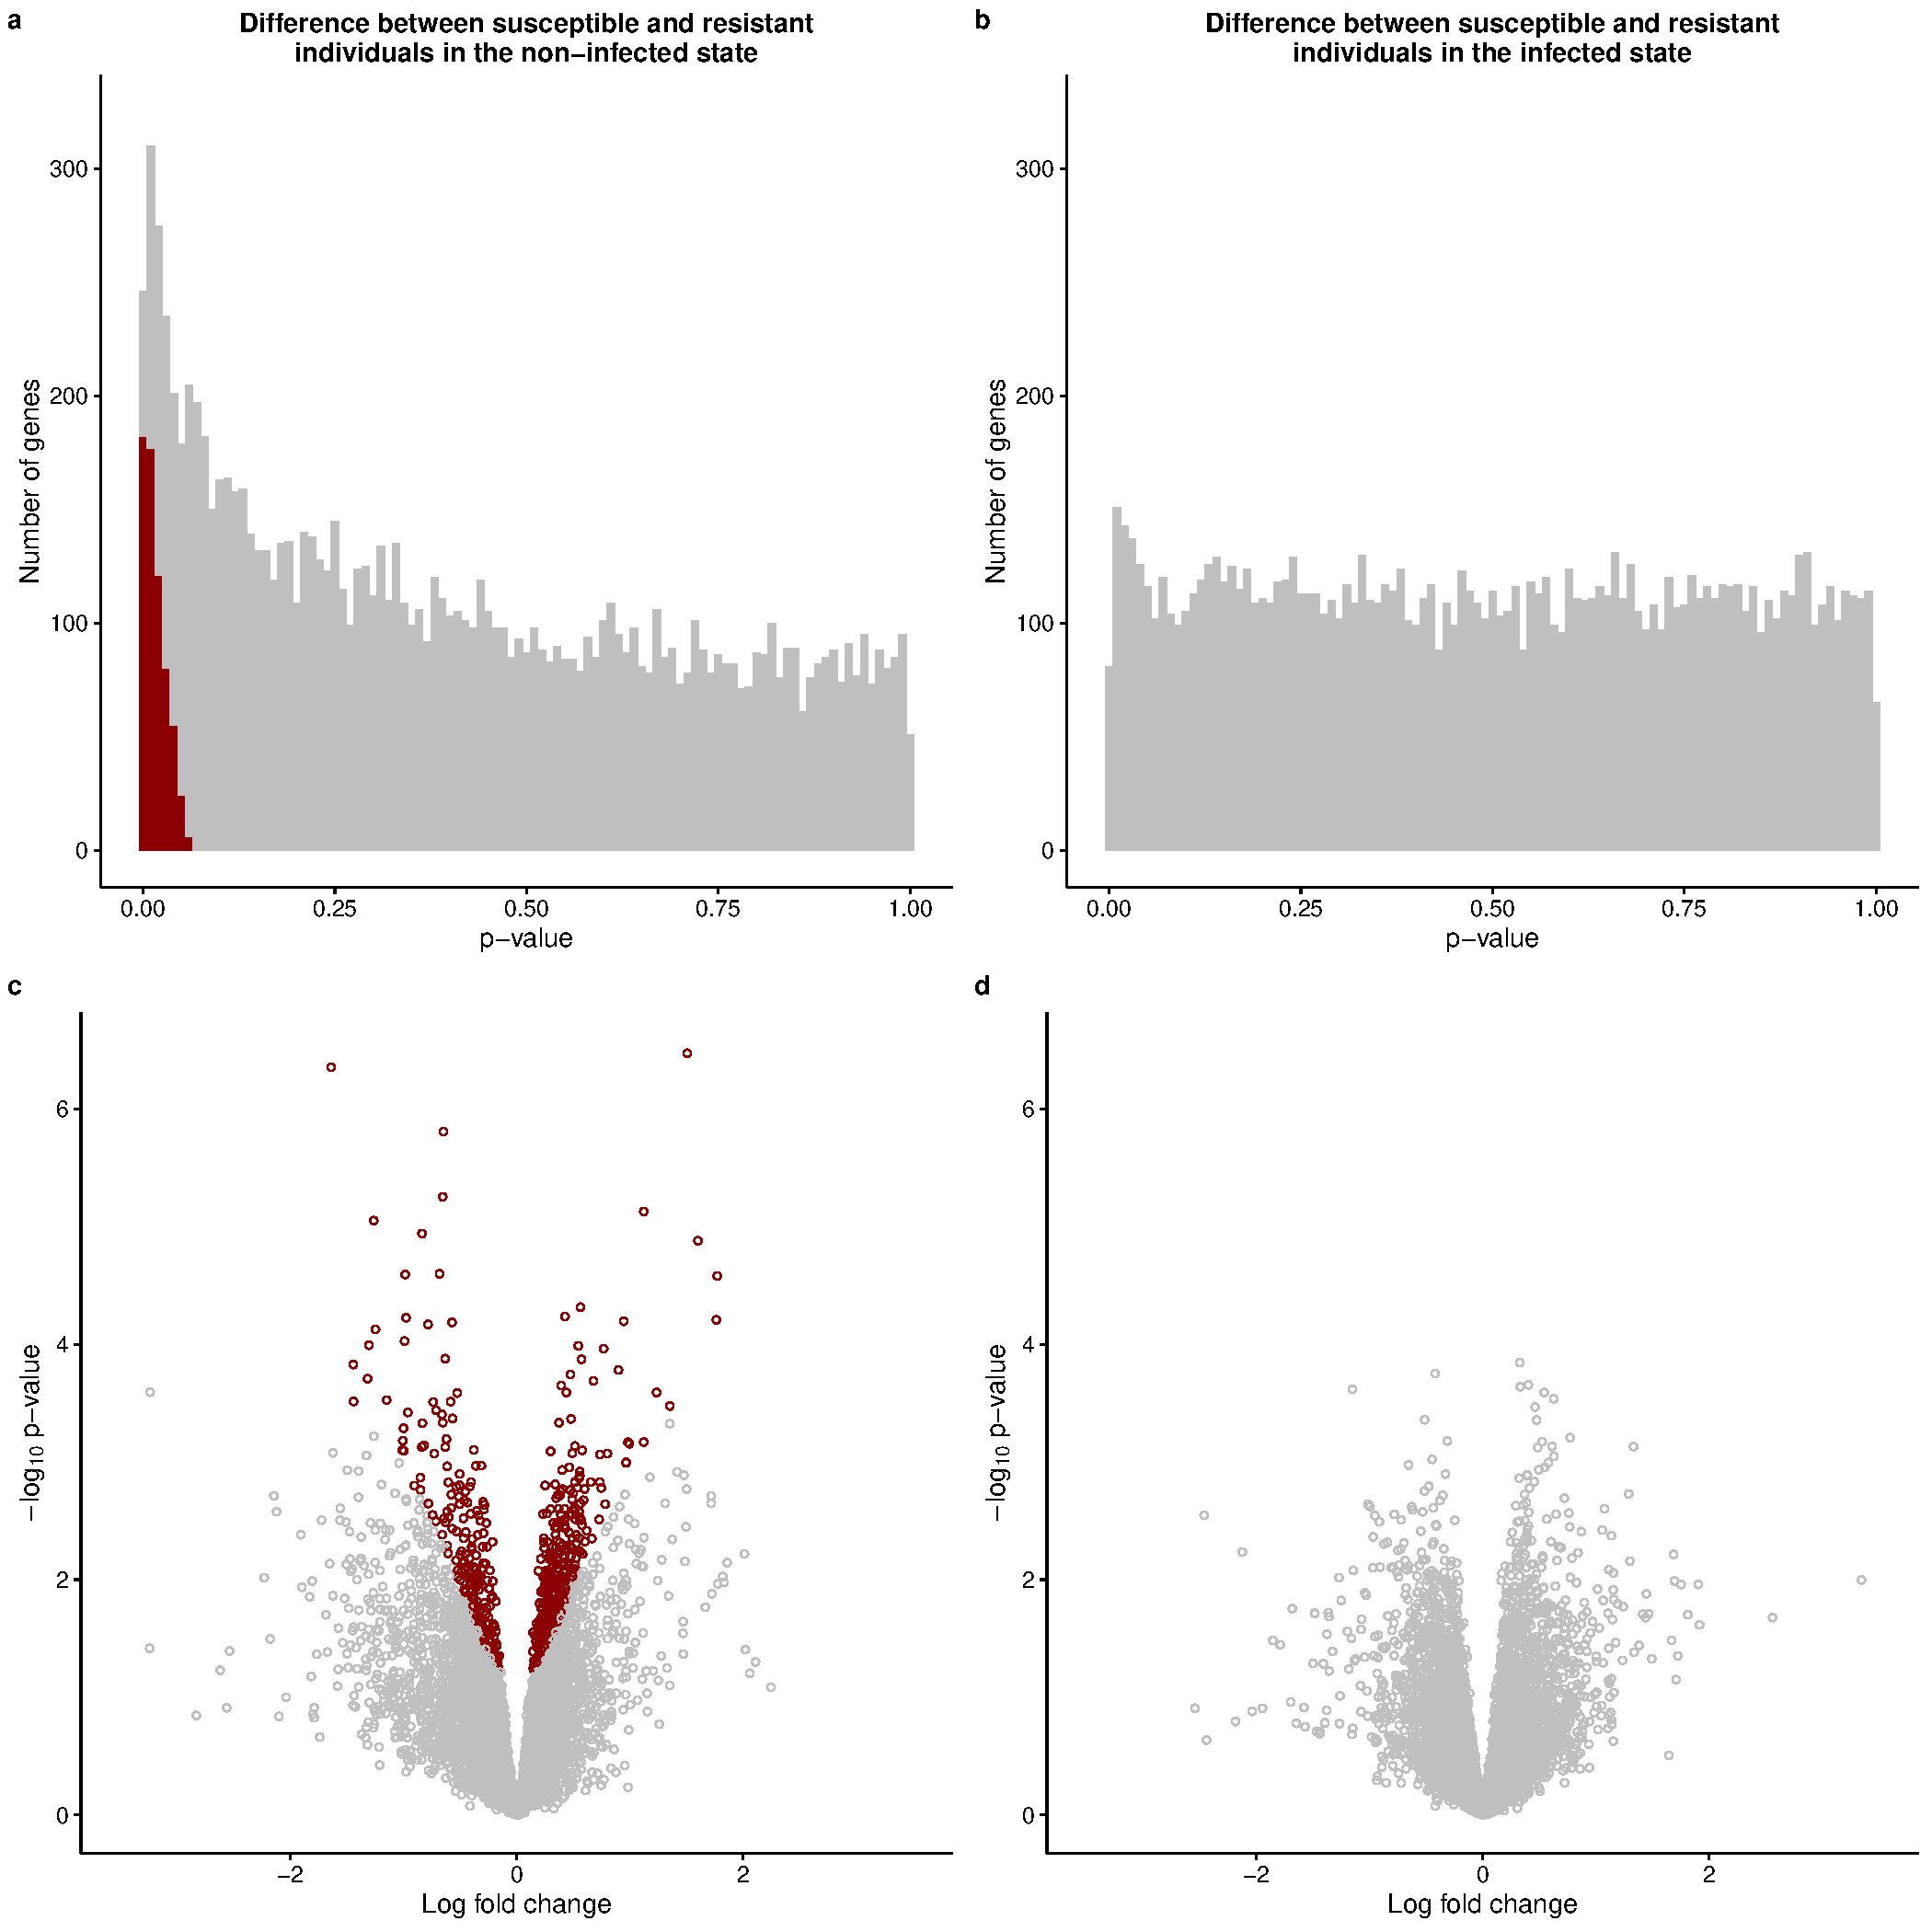
\includegraphics[width=\linewidth]{../figure/limma.pdf}
\caption{
Results of differential expression analysis. The top panels show the
distributions of unadjusted p-values for testing the null of no
differential expression between susceptible and resistant individuals
in the (a) non-infected or (b) infected state. The bottom panels show
the corresponding volcano plots for the (c) non-infected and (d)
infected states. The x-axis is the log fold change in gene expression
level between susceptible and resistant individuals and the y-axis is
the –log\textsubscript{10} p-value. Red indicates genes that are
classified as differentially expressed with a q-value less than 10\%.
}
\label{fig:limma}
\end{figure}
\subsection*{Differentially expressed genes are enriched with TB susceptibility loci}

We next sought evidence that genes classified as DE in our \emph{in
vitro} experimental system play a role in determining susceptibility
to TB. To do this, we intersected our data with results from TB
susceptibility GWAS conducted in Russia \cite{Curtis2015}, The Gambia
\cite{Thye2010}, Ghana \cite{Thye2010}, and Uganda and Tanzania
\cite{Sobota2016}. We also included data from a height GWAS conducted
in individuals of European ancestry \cite{LangoAllen2010} as a
negative control. To perform a combined analysis of our gene
expression data and the GWAS results, we had to define pairs of genes
(for which we have expression data) and SNPs (for which we obtained
GWAS \emph{P} values). Thus, each gene in our expression data was
coupled with the GWAS SNP with the lowest p-value among all tested
SNPs located within 50 kb of the gene’s transcription start site
(Supplementary Data S4; this gene-SNP definition was performed
separately for each GWAS data set).

Once we defined gene–SNP pairs, we asked whether differences in gene
expression levels between putatively resistant and susceptible
individuals could help us identify genetic variation that is
associated with susceptibility to TB. In other words, we asked whether
increasing evidence for DE genes is associated with low GWAS p-values.
To do so, we calculated the fraction of SNPs with a GWAS p-value lower
than 0.05 among SNPs that were paired with ranked subsets of genes
whose expression profiles show increasing effect size of expression
differences between putatively resistant and susceptible individuals.
In order to assess the significance of the observations, we performed
100 permutations of the enrichment analysis to derive an empirical
p-value.

Using this approach, we observed a clear enrichment (empirical
\emph{P} \textless \, 0.01) of low p-values for TB GWAS SNPs that are
paired with genes that are differentially expressed between
susceptible and resistant individuals in the non-infected state (Fig.
\ref{fig:gwas}a). In fact, we observed significant enrichments of
lower GWAS p values (empirical \emph{P} \textless \, 0.01) in all 4 TB
susceptibility GWAS (Russia, The Gambia, Ghana, Uganda and Tanzania)
(Supplementary Fig. \ref{fig:gwas-supp}) for all 4 differential
expression contrasts, namely resistant vs. susceptible individuals in
the non-infected state (Fig. \ref{fig:gwas}c), resistant vs.
susceptible individuals in the infected state (Fig. \ref{fig:gwas}d),
effect of treatment in resistant individuals (Fig. \ref{fig:gwas}e),
and effect of treatment in susceptible individuals (Fig.
\ref{fig:gwas}f). Reassuringly, we did not observe an enrichment of
low p values (empirical \emph{P} \textgreater \, 0.01) when we used
the same approach to consider data from the height GWAS (Fig.
\ref{fig:gwas}bcdef).


\begin{figure}[p]
\centering
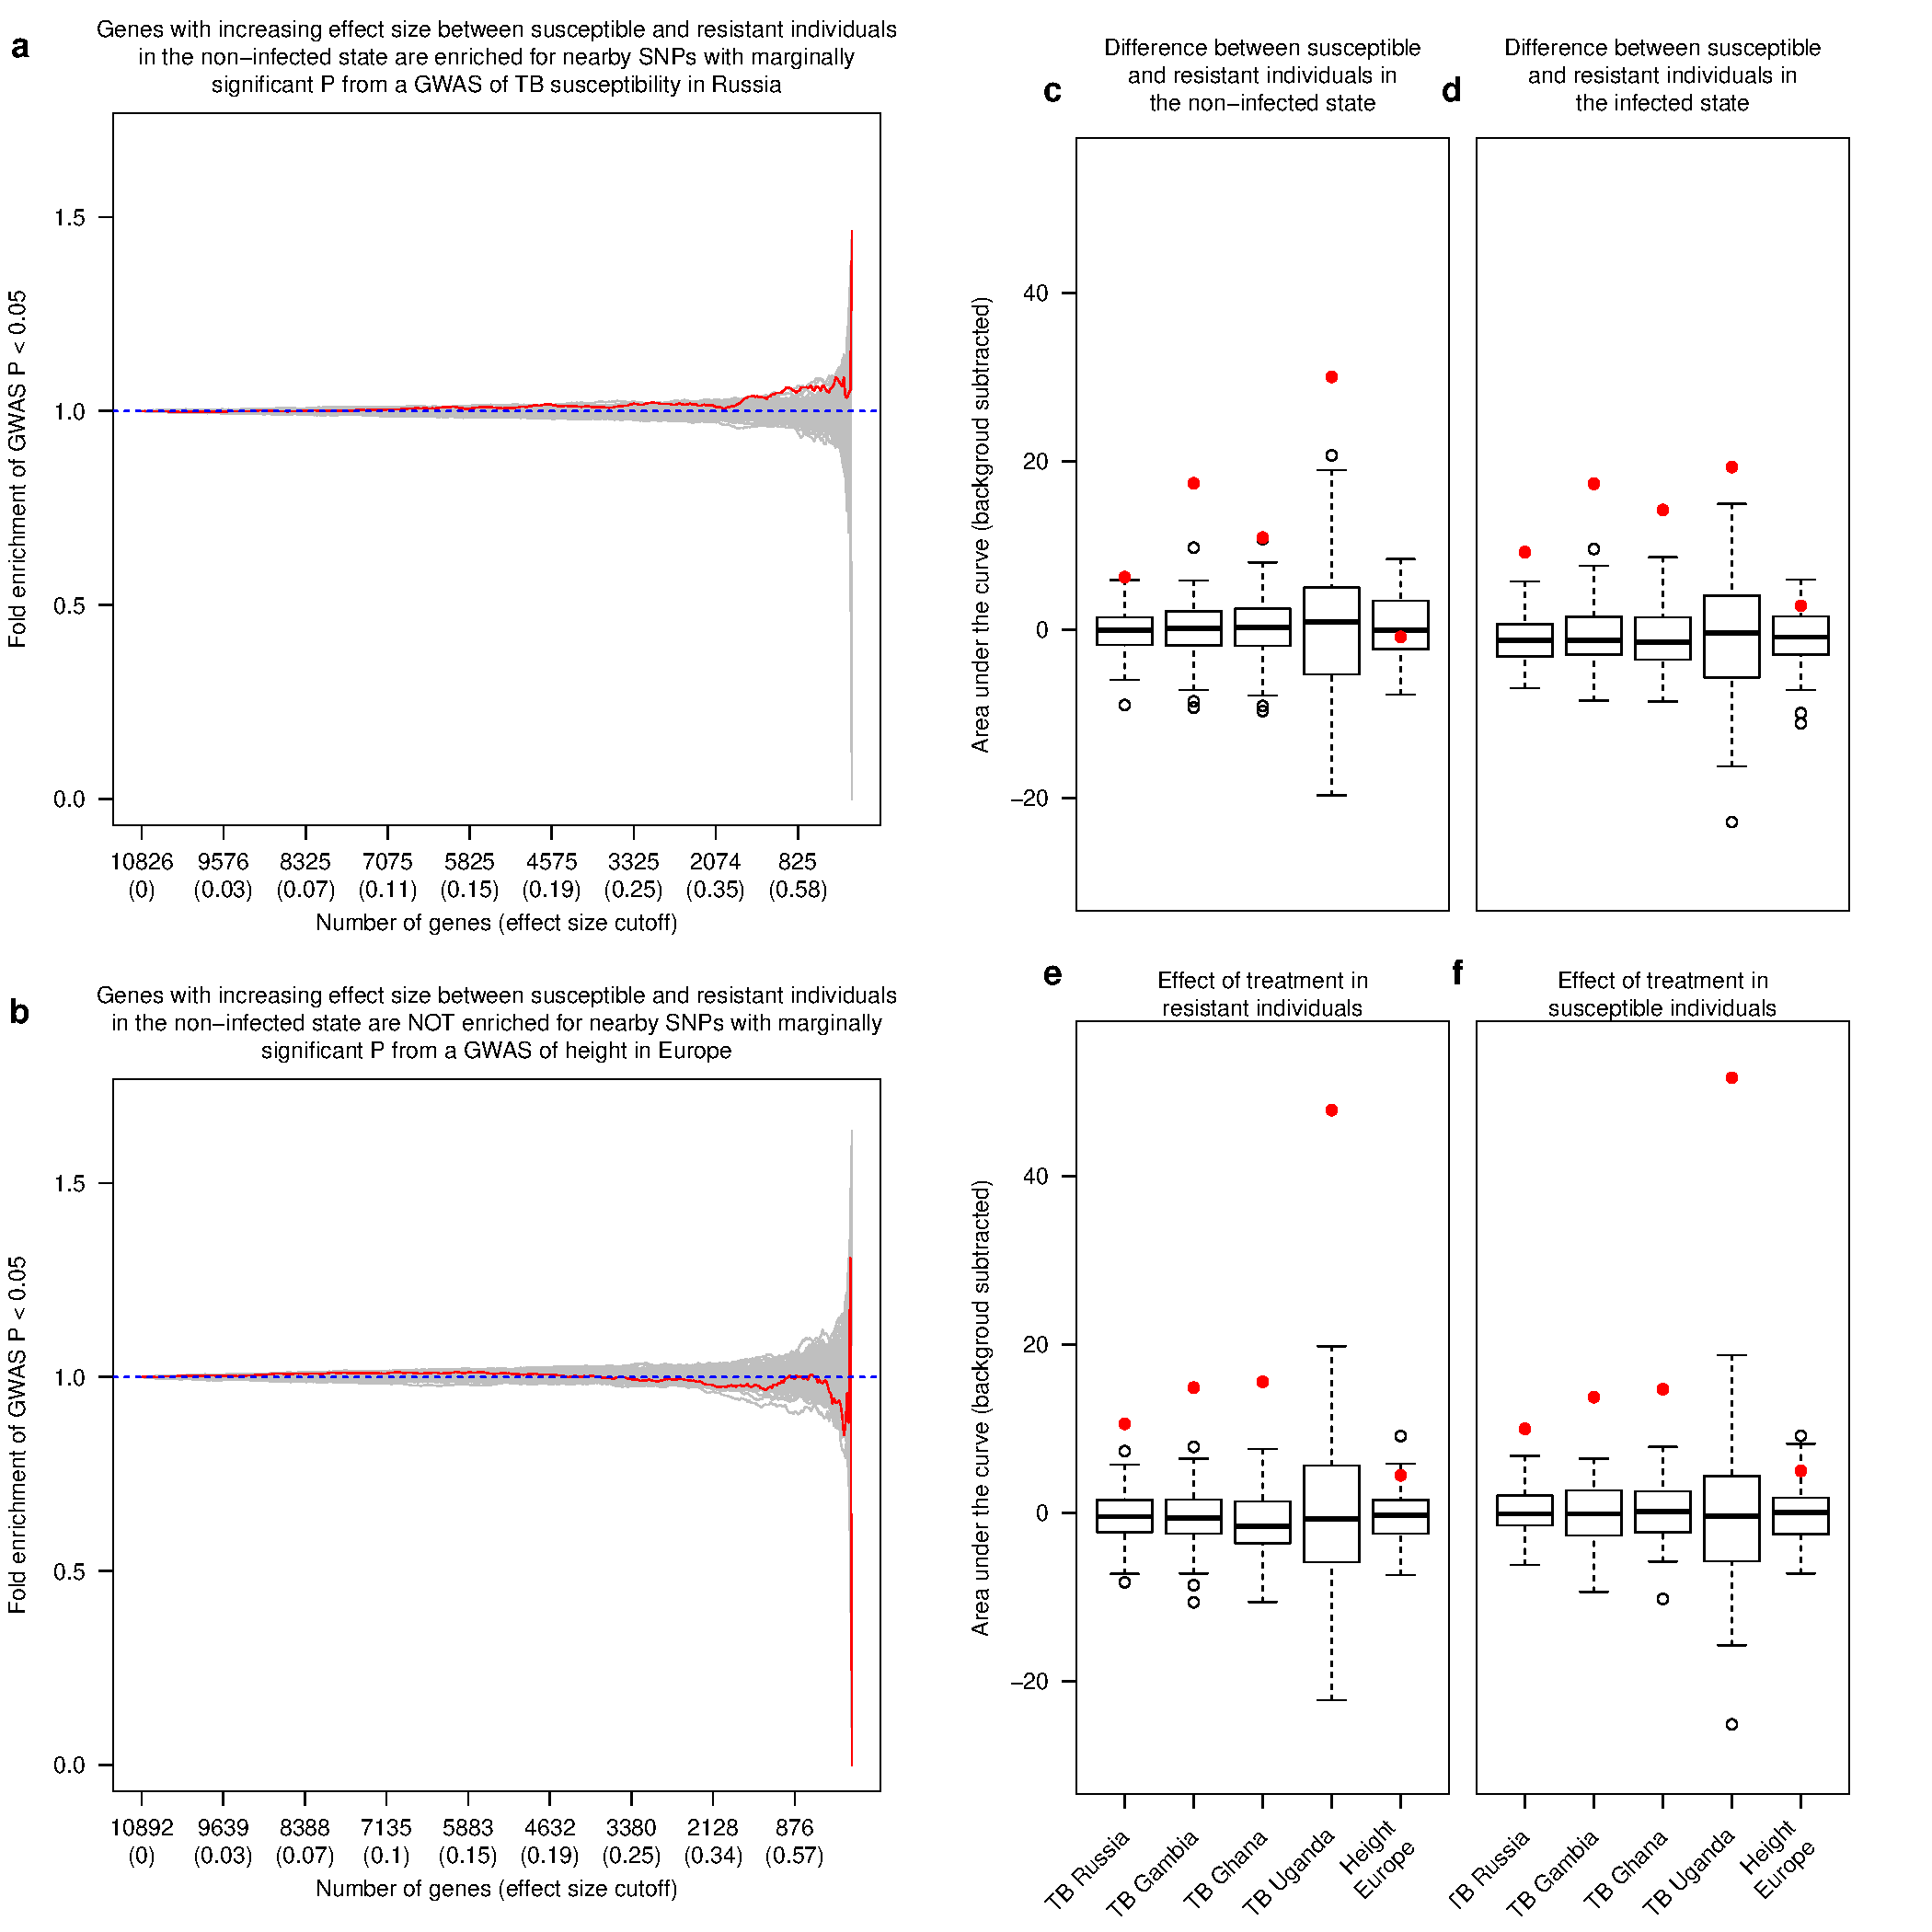
\includegraphics[width=\linewidth]{../figure/gwas-final.pdf}
\caption{
Comparison of differential expression and TB susceptibility GWAS
results. (a and b) The y-axis is the fold enrichment of SNPs with
p-value less than 0.05 from the (a) GWAS of TB susceptibility in
Russia \cite{Curtis2015} or (b) height in individuals of European
descent \cite{LangoAllen2010}. The x-axis is bins of genes with
increasingly stringent effect size cutoffs of the absolute expression
log fold change between putatively susceptible and resistant
individuals in the non-infected state. The effect size cutoffs were
chosen such that each bin from left to right contained approximately
25 fewer genes. The red line shows the results from the actual data.
The grey lines are the results from 100 permutations. The dashed blue
line at y=1 represents the null expectation. (c-f) Boxplots of the
area under the curve of the fold enrichment (red line in a and b)
minus the background level (blue y = 1 line in a and b) for each of
the 5 GWAS \cite{Curtis2015, Thye2010, Sobota2016} considered for the
4 differential expression contrasts: (c) resistant vs. susceptible
individuals in the non-infected state, (d) resistant vs. susceptible
individuals in the infected state, (e) effect of treatment in
resistant individuals, (f) effect of treatment in susceptible
individuals. The boxplot is the result of the 100 permutations, and
the red point is the result from the actual data. As a reference, the
leftmost boxplot in (c) corresponds to the enrichment plot in (a), and
the rightmost boxplot in (c) corresponds to the enrichment plot in
(b).
}
\label{fig:gwas}
\end{figure}

\subsection*{Susceptibility status can be predicted based on gene expression data}

Next we attempted to build a gene expression-based classifier to
predict TB susceptibility status (Supplementary Data S5). We focused
on the gene expression levels measured in the non-infected state both
because this is where we observed the largest gene regulatory
differences between putatively susceptible and resistant individuals
(Fig. \ref{fig:limma}ac), and also because, from the perspective of an
ultimate translational application, it is more practical to obtain
gene expression data from non-infected DCs. We trained a support
vector machine using the 99 genes that were differentially expressed
between resistant and susceptible individuals in the non-infected
state at a q-value less than 5\% (see Methods for a full description
of how we selected this model). Encouragingly, we observed a clear
separation between putatively susceptible and resistant individuals
when comparing the predicted probability of being susceptible to TB
for each sample obtained from leave-one-out-cross-validation (Fig.
\ref{fig:classifier}a). Using a cutoff of 0.25 for the predicted
probability of being susceptible to TB, we obtained a sensitivity of
100\% (5 out of 5 susceptible individuals classified as susceptible),
a specificity of \texttildelow88\% (15 out of 17 resistant individuals
classified as resistant), and a positive predictive value (PPV) of
\texttildelow71\% (5 of 7 individuals classified as susceptible were
susceptible).

Unfortunately our current data set is too small to properly split into
separate training and testing sets (it is challenging to collect
samples from previous TB patients, who are healthy and have no medical
reason to go back for a GP visit). To our knowledge, there are also no
other suitable data sets available with which to test out classifier
(that said, see Supplementary Fig. \ref{fig:class-svm-thuong} for the
results of applying the classifier to a non-ideal data set, which
measured gene expression in macrophages from a small number of
individuals \cite{Thuong2008}). Thus, in order to further assess the
plausibility of our model, we applied the classifier to data from an
independent study, which collected genome-wide gene expression levels
in DCs from 65 healthy individuals \cite{Barreiro2012}, none with a
previous history of TB. Using the cutoff of 0.25 for the probability
of being susceptible to TB (determined to be optimal in the training
set), \texttildelow11\% (7 of 65) of the individuals were classified
as susceptible to TB (Fig. \ref{fig:classifier}b). Adjusting for the
PPV obtained from the training set (\texttildelow71\%), our model
predicted that \texttildelow7.7\% of the healthy individuals were
susceptible. While we cannot confirm this result (the true
susceptibility status of these 65 individuals is unknown), this
observation is encouraging because our estimate is similar to the
commonly used inference that roughly 10\% of the general population is
susceptible to TB.

\begin{figure}[ht]
\centering
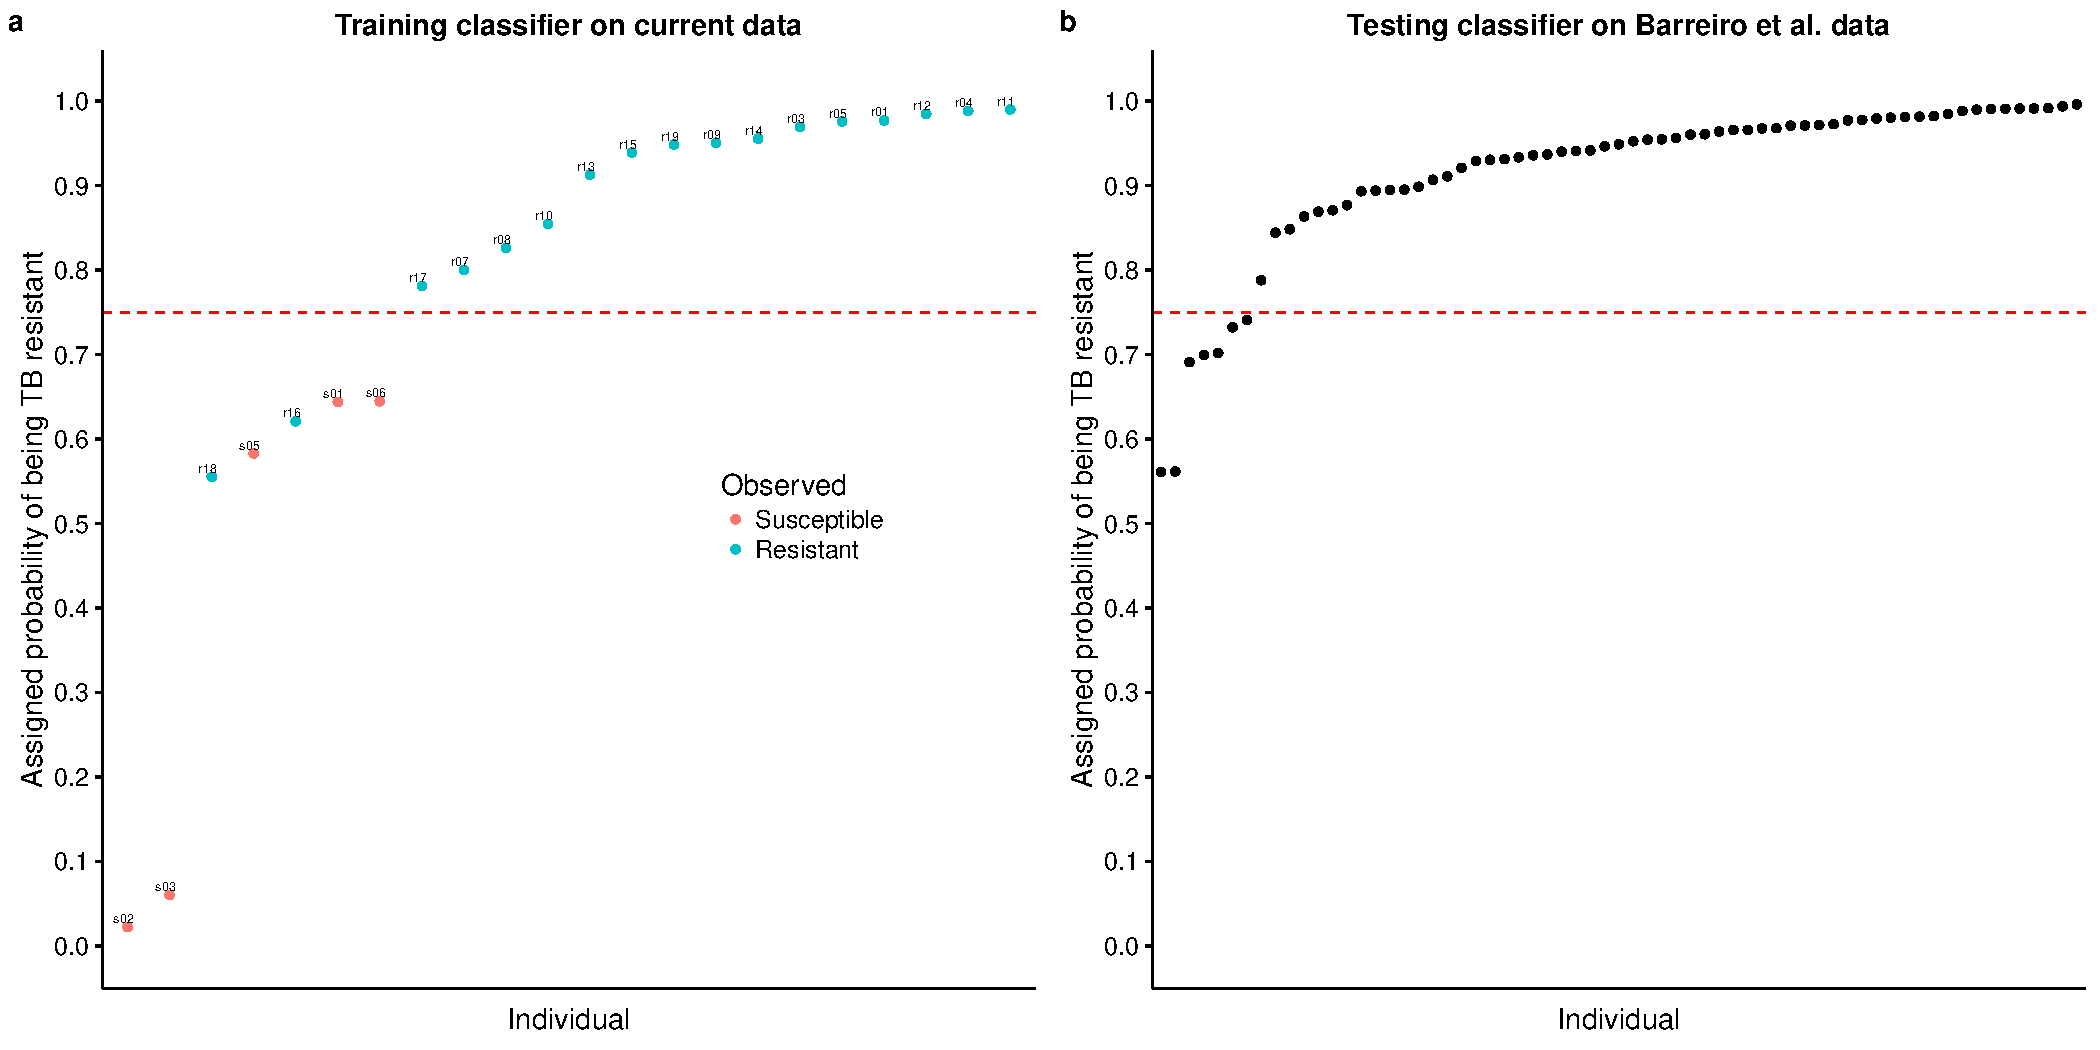
\includegraphics[width=\linewidth]{../figure/classifier-svm.pdf}
\caption{
Classifying TB susceptible individuals using a support vector machine
model. (a) The estimates of predicted probability of TB susceptibility
from the leave-one-out-cross-validation for individuals in the current
study. The blue circles represent individuals known to be susceptible
to TB, and orange those resistant to TB. The horizontal dashed red
line at a probability of 0.25 separates susceptible and resistant
individuals. (b) The estimates of predicted probability of TB
susceptibility from applying the classifier trained on the data from
the current study to a test set of independently collected healthy
individuals \cite{Barreiro2012}.
}
\label{fig:classifier}
\end{figure}

\section*{Discussion}

We obtained dendritic cells (DCs) from individuals that were known to
be putatively susceptible or resistant to developing active
tuberculosis (TB) and measured genome-wide gene expression levels in
non-infected DCs and DCs infected with \emph{Mycobacterium
tuberculosis} (MTB) for 18 hours. As expected, there were large
changes in gene expression due to MTB infection in the DCs from both
putatively resistant and susceptible individuals (Supplementary Fig.
\ref{fig:limma-supp}). We identified 645 genes which were
differentially expressed (DE) between susceptible and resistant
individuals in the non-infected state; whereas, we did not observe any
DE genes between susceptible and resistant individuals in the infected
state (Fig. \ref{fig:limma}). This suggests that the differences in
the transcriptomes between DCs of resistant and susceptible
individuals are present pre-infection. Yet, 18 hours after infection
gene expression profiles in both susceptible and resistant individuals
have converged to a similar gene regulatory network, presumably to
fight the infection. We confirmed that the absence of DE genes in the
infected state is \textbf{not} caused by a decrease in statistical
power due to an overall increase in gene expression variance upon
infection (Supplementary Fig. \ref{fig:variance}). We chose to measure
gene expression 18 hours post-infection because this time point was
previously associated with a large change in genome-wide gene
expression levels \cite{Tailleux2008}. Given our observations,
however, future studies investigating the difference in the innate
immune response between individuals resistant and susceptible to TB
may want to focus on earlier time points post-infection.

It is important to note that our study was not designed to uncover the
mechanisms underlying susceptibility or resistance to TB, but to try
and find a gene regulatory signature that might allow us to classify
individuals as either susceptible or resistant. That said, among the
645 DE genes between resistant and susceptible individuals in the
non-infected state, there were many interesting genes involved in
important innate immune activities critical for fighting MTB and other
pathogens such as autophagy \cite{Deretic2014, Castrejon-Jimenez2015},
phagolysosomal acidification, and antigen processing. In particular,
\emph{FEZ2}, a suppressor of autophagosome formation \cite{Spang2014},
was down-regulated when DCs were infected with MTB; however, in the
non-infected DCs, this gene has elevated expression level in
susceptible compared with resistant individuals. In turn,
\emph{ATP6V1B2}, a gene coding for a subunit of the proton transporter
responsible for acidifying phagolysosomes \cite{Sturgill-Koszycki1994,
Hornef2002, Hestvik2005}, has increased expression in susceptible
individuals compared to resistant in the non-infected state. Lastly,
genes coding for nine subunits of the proteasome, which is critical
for processing of MTB antigens to be presented via major
histocompatibility complex (MHC) class I molecules \cite{Flynn1992,
Grotzke2009, Grotzke2010, LindestamArlehamn2014}, have increased
expression in susceptible individuals compared to resistant in the
non-infected state. These genes are candidates for future functional
studies investigating the mechanisms of TB susceptibility.

We observed that DE genes in our \emph{in vitro} experimental system
were enriched for lower GWAS p-values (Fig. \ref{fig:gwas}). This
suggests that such \emph{in vitro} approaches are informative for
interrogating the genetic basis of disease susceptibility. That being
said, we recognize a major caveat with this analysis is that assigning
SNPs to their nearest gene on the linear chromosome is problematic
because regulatory variants can have longer range effects.
Nevertheless, considering this limitation, it was encouraging that we
were able to detect evidence of the genetic basis of TB susceptibility
in this system.

Not only did this analysis identify a global enrichment of TB
susceptibility loci, but by intersecting the expression and GWAS data,
we were able to identify a few interesting candidate genes, which were
only marginally significant in the original GWAS (Supplementary Data
S4). Here we highlight two genes (\emph{CCL1} and \emph{UNC13A}),
which have been previously shown to play important roles in MTB
infection. \emph{CCL1} is a chemokine that stimulates migration of
monocytes \cite{Miller1992}. In our study, it was upregulated in
susceptible individuals compared to resistant in both the non-infected
and infected states (but did not reach statistical significance in
either) and was statistically significantly upregulated with MTB
treatment. Furthermore, the nearby SNP assigned to \emph{CCL1} had a
p-value less than 0.01 in the TB susceptibility GWAS from The Gambia
and Ghana. A previous differential expression study of TB
susceptibility (discussed in more detail below) found that \emph{CCL1}
was upregulated to a greater extent 4 hours post-infection with MTB in
macrophages isolated from individuals with active TB (i.e.
susceptible) compared to individuals with latent TB (i.e. resistant)
\cite{Thuong2008}. Additionally they performed a candidate gene
association study and found that SNPs nearby \emph{CCL1} were
associated with TB susceptibility. In our previous study, we
discovered that \emph{CCL1} was one of only 288 genes that were
differentially expressed in macrophages 48 hours post-infection with
MTB and related mycobacterial species but not unrelated virulent
bacteria \cite{Blischak2015}. \emph{UNC13A} is involved in vesicle
formation \cite{Sudhof2004}. In our study, it was downregulated in
susceptible individuals compared to resistant in both the non-infected
and infected states (but did not reach statistical significance in
either) and was statistically significantly upregulated with MTB
treatment. Furthermore, the nearby SNP assigned to \emph{UNC13A} had a
p-value less than 0.01 in the TB susceptibility GWAS from Russia, The
Gambia, and Ghana. In our past study mapping expression quantitative
trait loci (eQTLs) in DCs 18 hours post-infection with MTB,
\emph{UNC13A} was one of only 98 genes which were associated with an
eQTL post-infection but not pre-infection, which we called
MTB-specific eQTLs \cite{Barreiro2012}. Thus our new results increased
the evidence that \emph{CCL1} and \emph{UNC13A} play important roles
in TB susceptibility.

Previous attempts to use gene expression based classifiers in the
context of TB have focused on predicting the status of an infection
rather than the susceptibility status of an individual
\cite{Berry2010, OGarra2013, Blankley2014}. In other words, the goal
of most previous studies was to detect individuals in the early stages
of active TB when antibiotic intervention would be most effective or
to monitor the effectiveness of a treatment regimen
\cite{Maertzdorf2015}. In contrast, our goal was not to distinguish
between active and latent TB, but instead to be able to determine
susceptibility status before individuals are infected with MTB. Even
with our small sample size, we were able to successfully train a
classier with high sensitivity and decent specificity. Because such a
classification of susceptibility status could affect the decision of
whether or not to take antibiotics to treat latent TB
\cite{Munoz2015}, false negatives (susceptible individuals mistakenly
classified as resistant) would be much more harmful than false
positives (resistant individuals mistakenly classified as
susceptible). For that reason, we emphasized sensitivity over
specificity.

To our knowledge, our study was only the second to collect data from
\emph{in vitro} MTB-infected innate immune cells isolated from
individuals known to be putatively susceptible to MTB (Thuong et al.,
2008). However, there were substantial differences between our study
and that of Thuong et al., 2008 \cite{Thuong2008}. First, they derived
and infected macrophages, the primary target host cell in which MTB
resides; whereas, we derived and infected DCs, which play a larger
role in stimulating the adaptive immune response to MTB. Second, we
collected samples from a larger number of putatively resistant
individuals (19 versus 4), increasing our power to distinguish between
the gene expression profiles of susceptible and resistant individuals.
Third, they measured gene expression with microarrays; whereas, we
used RNA-sequencing. Considering the substantial technical differences
between the methods used and the biological differences between DCs
and macrophages \cite{Chaussabel2003,Tailleux2008}, unsurprisingly, we
were unable to identify the susceptible individuals from Thuong et
al., 2008 \cite{Thuong2008} using our classifier (Supplementary Fig.
\ref{fig:class-svm-thuong}).

Indeed, at this time, we are not aware of any other data set from
healthy individuals known to be sensitive to TB, with which we can
further test our classifier. When we applied our classifier to an
independent set of non-infected DCs isolated from healthy individuals
of unknown susceptibility status, our model predicted that
\texttildelow7.7-11\% of the individuals were susceptible to TB, which
reassuringly is similar to the average in the general population
(10\%). Despite this, our results must be interpreted cautiously; at
best as a proof-of-principle, due to our very small sample size of
only 5 susceptible individuals. That said, our promising results in
this small study suggest that collecting blood samples from a larger
cohort of susceptible individuals would enable building a gene
expression based classifier able to confidently assess risk of TB
susceptibility. By reducing the number of resistant individuals
receiving treatment for latent TB, we can eliminate the adverse health
effects of a 6 month regimen of antibiotics for these individuals and
also reduce the selective pressures on MTB to develop drug resistance.
\section*{Methods}

\subsection*{Ethics statement}

We recruited 25 subjects to donate a blood sample for use in our
study. All methods were carried out in accordance with relevant
guidelines and regulations. All participants gave written informed
consent in accordance with the Declaration of Helsinki principles.
Peripheral human blood was collected from patients at ICAReB platform
of Institut Pasteur Paris and at the Centre for Infectious Disease
Prevention, University hospital Caen. The Protocol has been approved
by French Ethical Committee (CPP North Ouest III, n° A12 - D33
-VOL.13), and by the Institutional Review Boards of the University of
Chicago (10-504-B) and the Institut Pasteur (IRB00006966).
\subsection*{Sample collection}

We collected whole blood samples from healthy Caucasian male
individuals living in France. The putatively resistant individuals
tested positive for latent TB in an interferon-$\gamma$ release assay,
but had never developed active TB. The putatively sensitive
individuals had developed active TB in the past, but were currently
healthy.
\subsection*{Isolation and infection of dendritic cells}

We performed these experiments as previously described
\cite{Barreiro2012}. Briefly, we isolated mononuclear cells from the
whole blood samples using Ficoll-Paque centrifugation, extracted
monocytes via CD14 positive selection, and differentiated the
monocytes into dendritic cells (DCs) by culturing them for 5 days in
RPMI 1640 (Invitrogen) supplemented with 10\% heat-inactivated FCS
(Dutscher), L-glutamine (Invitrogen), GM-CSF (20 ng/mL; Immunotools),
and IL-4 (20 ng/mL; Immunotools). Next we infected the DCs with
\emph{Mycobacterium tuberculosis} (MTB) H37Rv at a multiplicity of
infection of 1-to-1 for 18 hours.
\subsection*{RNA extraction and sequencing}

We extracted RNA using the Qiagen miRNeasy Kit and prepared sequencing
libraries using the Illumina TruSeq Kit. We sent the master mixes to
the University of Chicago Functional Genomics Facility to be sequenced
on an Illumina HiSeq 4000. We designed the batches for RNA extraction,
library preparation, and sequencing to balance the experimental
factors of interest and thus avoid potential technical confounders
(Supplementary Fig. \ref{fig:process}).
\subsection*{Read mapping}

We mapped reads to human genome hg38 (GRCh38) using Subread
\cite{Liao2013} and discarded non-uniquely mapping reads. We
downloaded the exon coordinates of 19,800 Ensembl \cite{Yates2016}
protein-coding genes (Ensembl 83, Dec 2015, GRCh38.p5) using the
R/Bioconductor \cite{Huber2015} package biomaRt \cite{Durinck2005,
Durinck2009} and assigned mapped reads to these genes using
featureCounts \cite{Liao2014}.
\subsection*{Quality control}

First we filtered genes based on their expression level by removing
all genes with a transformed median log\textsubscript{2} counts per
million (cpm) of less than zero. This step resulted in a set of 11,336
genes for downstream analysis (Supplementary Fig. \ref{fig:gene},
Supplementary Data S2). Next we used principal components analysis
(PCA) and hierarchical clustering to identify and remove 6 outlier
samples (Supplementary Fig. \ref{fig:heat-all}, \ref{fig:heat-filt},
\ref{fig:outliers}). We did this systematically, by removing any
sample whose data projections did not fall within two standard
deviations of the mean for any of the first six PCs (for the first PC,
which separated the samples by treatment, we calculated a separate
mean for the non-infected and infected samples).

After filtering lowly expressed genes and removing outliers, we
performed the PCA again to check for any potential confounding
technical batch effects (Supplementary Fig. \ref{fig:batch}).
Reassuringly, the major sources of variation in the data were from the
biological factors of interest. PC1 was strongly correlated with the
effect of treatment, and PCs 2-6 were correlated with inter-individual
variation. The only concerning technical factor was the infection
experiments, which were done in 12 separate batches (Supplementary
Fig. \ref{fig:process}). Infection batch correlated with PCs 3 and 5;
however, we verified that this variation was not confounded with our
primary outcome of interest, TB susceptibility (Supplementary Fig.
\ref{fig:infection}).
\subsection*{Differential expression analysis}

We used limma+voom \cite{Smyth2004, Law2014, Ritchie2015} to implement
the following linear model to test for differential expression:
\begin{equation} \label{eq:limma}
Y\ \sim \beta_{0} + X_{treat}\beta_{treat} + X_{status}\beta_{status} + X_{treat,status}\beta_{treat,status} + I + \epsilon
\end{equation}
where $\beta_{0}$ is the mean expression level in non-infected cells
of resistant individuals, $\beta_{treat}$ is the fixed effect of
treatment in resistant individuals, $\beta_{status}$ is the fixed
effect of susceptibility status in non-infected cells,
$\beta_{treat,status}$ is the fixed interaction effect of treatment in
susceptible individuals (i.e. modeling the interaction between
treatment and susceptibility status), and $I$ is the random effect of
individual. The random individual effect was implemented using the
limma function duplicateCorrelation \cite{Smyth2005}. To jointly model
the data with voom and duplicateCorrelation, we followed the
recommended best practice of running both voom and
duplicateCorrelation twice in succession \cite{Liu2015}.

We used the model to test different hypotheses (Supplementary Data
S3). We identified genes which were differentially expressed (DE)
between infected and non-infected DCs of resistant individuals by
testing $\beta_{treat} = 0$, genes which were DE between infected and
non-infected DCs of susceptible individuals by testing $\beta_{treat}
+ \beta_{treat,status} = 0$, genes which were DE between susceptible
and resistant individuals in the non-infected state by testing
$\beta_{status} = 0$, and genes which were DE between susceptible and
resistant individuals in the infected state by testing $\beta_{status}
+ \beta_{treat,status} = 0$. We corrected for multiple testing using
q-values estimated via adaptive shrinkage \cite{Stephens2016} and
considered differentially expressed genes as those with a q-value less
than 10\%.

Note that we also tested the interaction term, $\beta_{treat,status} =
0$, to identify genes in which the difference in expression level
between the infected and non-infected states was significantly
different between susceptible and resistant individuals. However, as
expected since no DE genes were identified between susceptible and
resistant individuals in the infected state (see Results), the results
of testing the interaction term were partially redundant with the
results of testing differences between susceptible and resistant
individuals in the non-infected state, and thus we ignored these
results throughout this study.
\subsection*{Combined analysis of gene expression data and GWAS results}

The GWAS p-values were from previously published studies of TB
susceptibility conducted in Russia \cite{Curtis2015}, The Gambia
\cite{Thye2010}, Ghana \cite{Thye2010}, and Uganda and Tanzania
\cite{Sobota2016} (and a height GWAS in individuals of European
descent \cite{LangoAllen2010}). To perform a combined analysis of the
gene expression and the summary statistics from each GWAS, we assigned
each gene to the SNP with the minimum GWAS p-value out of all the SNPs
located within 50 kb up or downstream of its transcription start site.
Specifically, we obtained the genomic coordinates of the SNPs with the
R/Bioconductor \cite{Huber2015} package
SNPlocs.Hsapiens.dbSNP144.GRCh38 and matched SNPs to nearby genes
using GenomicRanges \cite{Lawrence2013}. 10,265 to 11,060 of the
11,336 genes were assigned an association p-value depending on the
GWAS (Supplementary Data S4). For each of the 4 differential
expression contrasts we tested (resistant vs. susceptible individuals
in the non-infected state, resistant vs. susceptible individuals in
the infected state, effect of treatment in resistant individuals,
effect of treatment in susceptible individuals), we also performed an
enrichment analysis. To do so, we calculated the fraction of genes
assigned a GWAS SNP with p-value less than 0.05 for bins of genes
filtered by increasingly stringent cutoffs for the observed
differential expression effect size (the absolute value of the log
fold change). The effect size cutoffs were chosen such that on average
each subsequent bin differed by 25 genes. To measure enrichment, we
calculated the area under the curve using the R package flux
\cite{Jurasinski2014} (we also subtracted the background area under
the line y = 1 because the number of genes assigned a SNP varied
across the GWAS). In order to assess significance, we calculated the
area under the curve for 100 permutations of the data. All
differential expression tests were statistically significantly
enriched for SNPs with low GWAS p-values in every TB susceptibility
GWAS (empirical \emph{P} \textless \, 0.01) and not enriched for the
height GWAS (empirical \emph{P} \textgreater \, 0.01) (Fig.
\ref{fig:gwas}; Supplementary Fig. \ref{fig:gwas-supp}).
\subsection*{Classifier}

The training set included data from the 44 high-quality non-infected
samples from this study with known susceptibility status. The test set
included the 65 non-infected samples from one of our previous studies
in which the susceptibility status is unknown \cite{Barreiro2012}, and
thus assumed to be similar to that in the general population
(\texttildelow10\%) (we also tested the classifier on data from a
small study of macrophages \cite{Thuong2008}, Supplementary Fig.
\ref{fig:class-svm-thuong}). Because the two studies are substantially
different, we took multiple steps to make them comparable. First, we
subset to include only those 9,450 genes which were assayed in both.
Second, because the dynamic range obtained from RNA-seq (current
study) and microarrays (previous study \cite{Barreiro2012}) were
different, we normalized the gene expression levels to a standard
normal ($\mu = 0$, $\sigma = 1$) distribution (Supplementary Fig.
\ref{fig:combined-dist}; note however that this strategy is unable to
correct for the inability of microarrays to accurately quantify genes
with expression levels that result in fluorescence levels below the
background level or above the saturation limit). Third, we corrected
for the large, expected batch effect between the two studies by
regressing out the first PC of the combined expression data using the
limma function removeBatchEffect \cite{Ritchie2015} (Supplementary
Fig. \ref{fig:combined-pca}).

To identify genes to use in the classifier, we performed a
differential expression analysis on the normalized, batch-corrected
data from the current study using the same approach described above
(with the exception that we no longer used voom \cite{Law2014} since
the data were no longer counts). Specifically, we tested for
differential expression between susceptible and resistant individuals
in the non-infected state and identified sets of genes to use in the
classifier by varying the q-value cutoff. Cutoffs of 5\%, 10\%, 15\%,
20\%, and 25\% corresponded to gene set sizes of 99, 385, 947, 1,934,
and 3,697, respectively. We used the R package caret \cite{Kuhn2008}
to train 3 different machine learning models: elastic net
\cite{Friedman2010}, support vector machine \cite{Karatzoglou2004},
and random forest \cite{Liaw2002} (the parameters for each individual
model were selected using the Kappa statistic). To assess the results
of the model on the training data, we performed
leave-one-out-cross-validation (LOOCV). In order to choose the model
with the best performance, we calculated the difference between the
mean of the LOOCV-estimated probabilities of being TB resistant for
the samples known to be TB resistant and the corresponding mean for
the samples known to be TB susceptible. This metric emphasized the
ability to separate the susceptible and resistant individuals into two
separate groups. Using this metric, the best performing model was the
support vector machine with the 99 genes that are significantly
differentially expressed at a q-value of 5\% (Fig.
\ref{fig:classifier}a ,Supplementary Fig. \ref{fig:class-compare},
Supplementary Data S5); however, both the elastic net (Supplementary
Fig. \ref{fig:class-en}) and random forest (Supplementary Fig.
\ref{fig:class-rf}) had similar performance. Lastly, we tested the
classifier by predicting the probability of being TB susceptible in
the 65 healthy samples (Fig. \ref{fig:classifier}b). For evaluating
the predictions on the test set of individuals with unknown
susceptibility status, we used a relaxed cutoff of the probability of
being TB susceptible of 0.25, which was based on the ability of the
model at this cutoff to classify all TB susceptible individuals in the
training set as susceptible with only 2 false positives. As expected,
the 99 genes used in the classifier had similar normalized,
batch-corrected median expression levels in the non-infected state
across both studies (Supplementary Fig. \ref{fig:class-exp}).
\subsection*{Software implementation}

We automated our analysis using Python (https://www.python.org/) and
Snakemake \cite{Koster2012}. Our processing pipeline used the general
bioinformatics software FastQC
(http://www.bioinformatics.babraham.ac.uk/projects/fastqc/), MultiQC
\cite{Ewels2016}, samtools \cite{Li2009}, and bioawk
(https://github.com/lh3/bioawk). We used R \cite{R2015} for all
statistics and data visualization. We obtained gene annotation
information from the Ensembl \cite{Yates2016} and Lynx
\cite{Sulakhe2016} databases. The computational resources were
provided by the University of Chicago Research Computing Center. All
code is available for viewing and reuse at
https://github.com/jdblischak/tb-suscept.
\subsection*{Data availability}

The raw fastq files have been deposited in NCBI's Gene Expression
Omnibus \cite{Edgar2002} and are accessible through GEO Series
accession number GSE94116
(http://www.ncbi.nlm.nih.gov/geo/query/acc.cgi?acc=GSE94116). The
RNA-seq gene counts and other summary data sets are included as
Supplementary Data and are also available for download at
https://github.com/jdblischak/tb-suscept.

While a small subset of the GWAS summary statistics required for
partially reproducing our results were included in Supplementary Data
S4, we do not have permission to share the full set of summary
statistics from the previously published TB susceptibility GWAS that
would be required for fully reproducing our results. To access the
summary statistics, contact the authors directly: Russia - Sergey
Nejentsev (sn262@cam.ac.uk), Ghana and The Gambia - Thorsten Thye
(thye@bnitm.de), Uganda and Tanzania - Scott M. Williams
(smw154@case.edu). The summary statistics for the height GWAS can be
downloaded from the GIANT Consortium’s website
(http://portals.broadinstitute.org/collaboration/giant/index.php/GIANT\_consortium\_data\_files).
\section*{Acknowledgements}

We thank Matthew Stephens and John Novembre for providing feedback and
Gilad lab members for helpful discussion. We thank Marie-Noëlle
Ungeheuer for help recruiting subjects. We thank Sergey Nejentsev for
sharing data from the GWAS in Russia. We thank Thorsten Thye for
sharing data from the GWAS in Ghana and The Gambia. We thank Rafal S.
Sobota, Catherine M. Stein, Giorgio Sirugo, and Scott M. Williams for
sharing data from the GWAS in Uganda and Tanzania. This study was
funded by National Institutes of Health (NIH) Grant AI087658 to Y.G.
and L.T. J.D.B. was supported by NIH Grant T32GM007197. The content is
solely the responsibility of the authors and does not necessarily
represent the official views of the NIH.
\section*{Author contributions}

Y.G., L.T., and L.B.B. conceived of the study and designed the
experiments. C.C., E.B., A.D., G.M., O.C., C.V.P., J.H., and R.B.
collected samples. L.T. coordinated sample collection and performed
the infection experiments. M.M. extracted the RNA and prepared the
sequencing libraries. J.D.B. analyzed the results. L.B.B. and Y.G.
supervised the project. J.D.B. wrote the paper with input from Y.G.,
L.T., L.B.B, and R.B.
\section*{Competing interests}

The authors declare no competing financial interests.

\bibliography{references}

\clearpage\newpage
\beginsupplement
\section*{Supplementary information}

\subsection*{Supplementary figures}


\begin{figure}[ht]
\centering
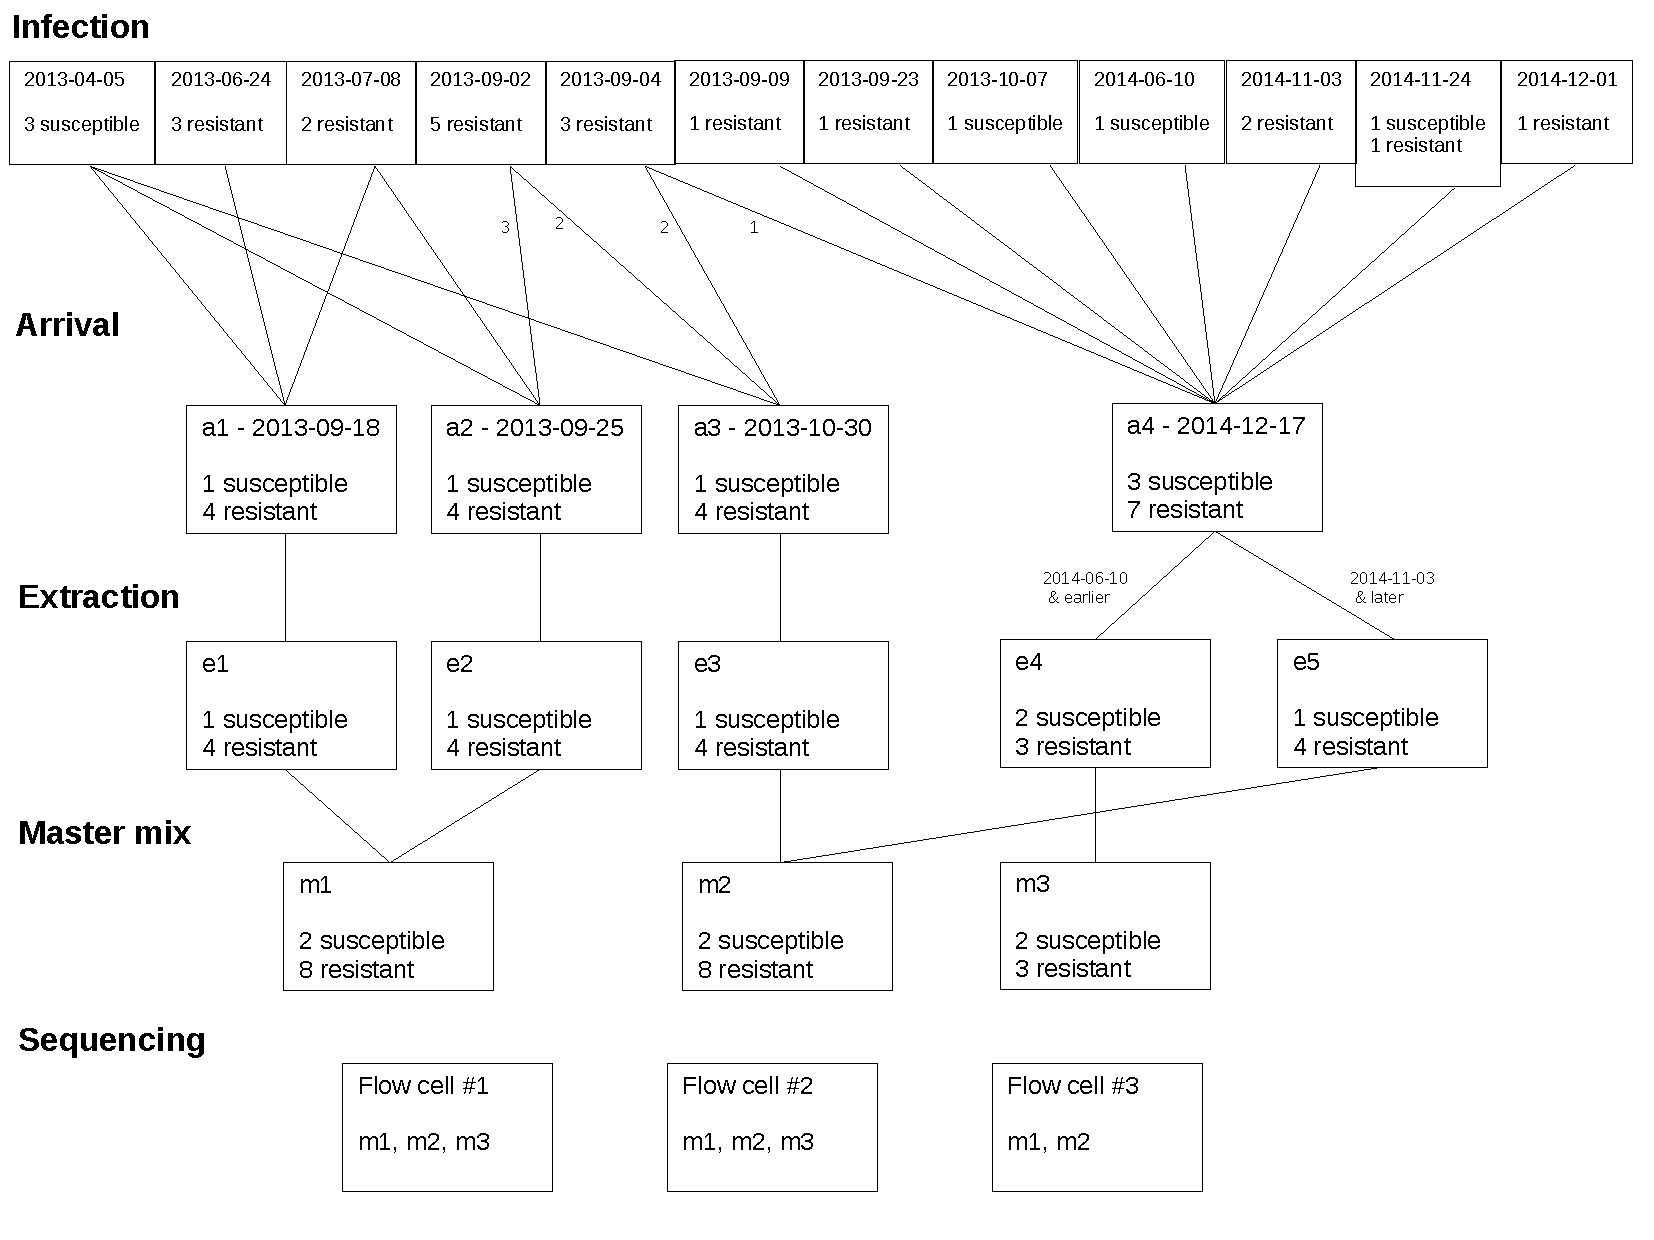
\includegraphics[width=\linewidth]{../figure/processing.pdf}
\caption{
Batch processing. We designed the processing of the samples to
minimize the introduction of technical batch effects. Specifically, we
attempted to balance the processing of samples obtained from
susceptible and resistant individuals. In the diagram, each box
represents a batch. “Infection” labels the batches of the infection
experiments, “Arrival” labels the batch shipments of cell lysates
arrived in Chicago, USA from Paris, France, “Extraction” labels the
batches of RNA extraction, “Master Mix” labels the batches of library
preparation, and “Sequencing” labels the batches of flow cells. Each
master mix listed in a flow cell batch was sequenced on only one lane
of that flow cell.
}
\label{fig:process}
\end{figure}


\begin{figure}[ht]
\centering
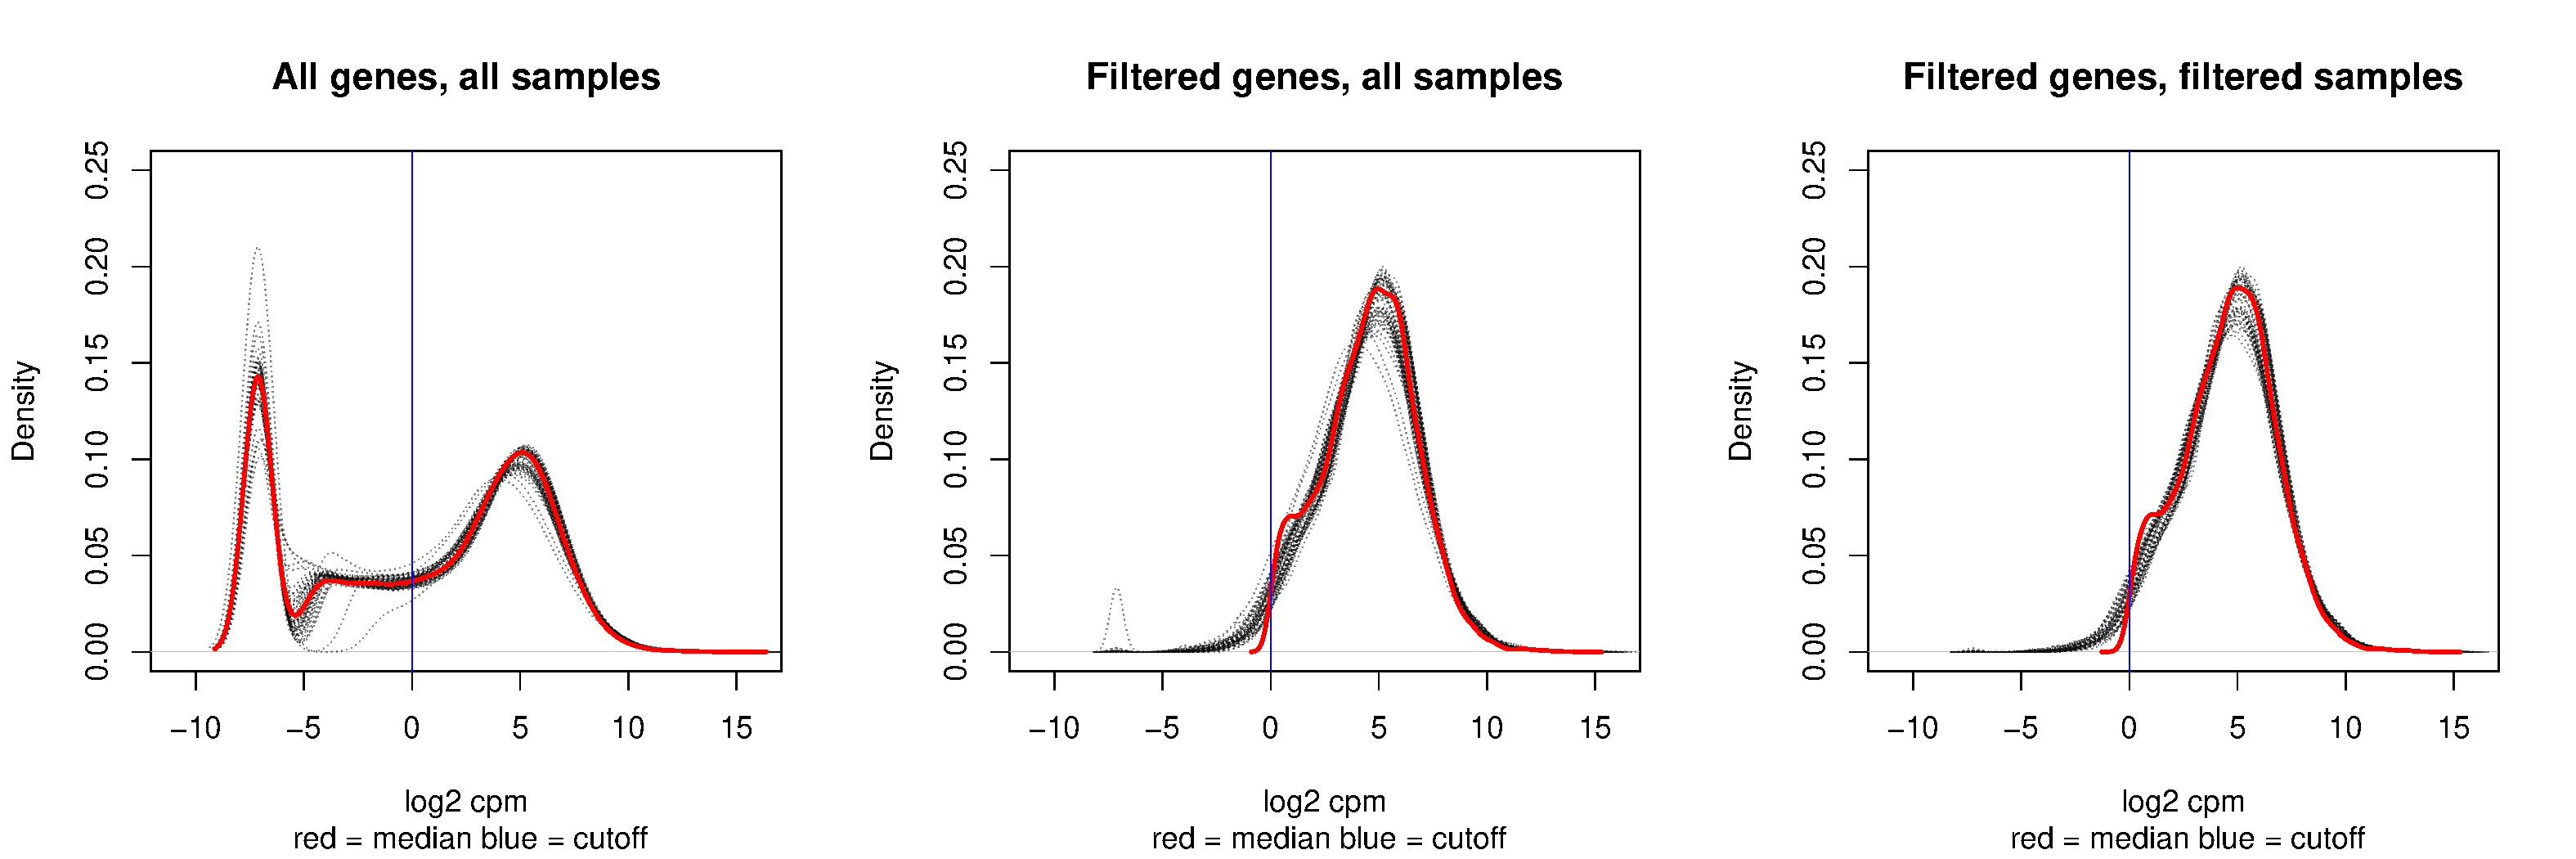
\includegraphics[width=\linewidth]{../figure/gene-exp-distribution.pdf}
\caption{
Gene expression distributions before and after filtering genes and
samples. The log\textsubscript{2} counts per million (cpm) of each
sample is plotted as a dashed gray line. The solid red line represents
the median value across all the samples. The vertical solid blue line
at $x = 0$ represents the cutoff used to filter lowly expressed genes
based on their median log\textsubscript{2} cpm. The left panel is the
data from all 19,800 genes and 50 samples, the middle panel is the
data from the 11,336 genes remaining after removing lowly expressed
genes, and the right panel is the data from 11,336 genes and the 44
samples remaining after removing outliers.
}
\label{fig:gene}
\end{figure}

\begin{figure}[ht]
\centering
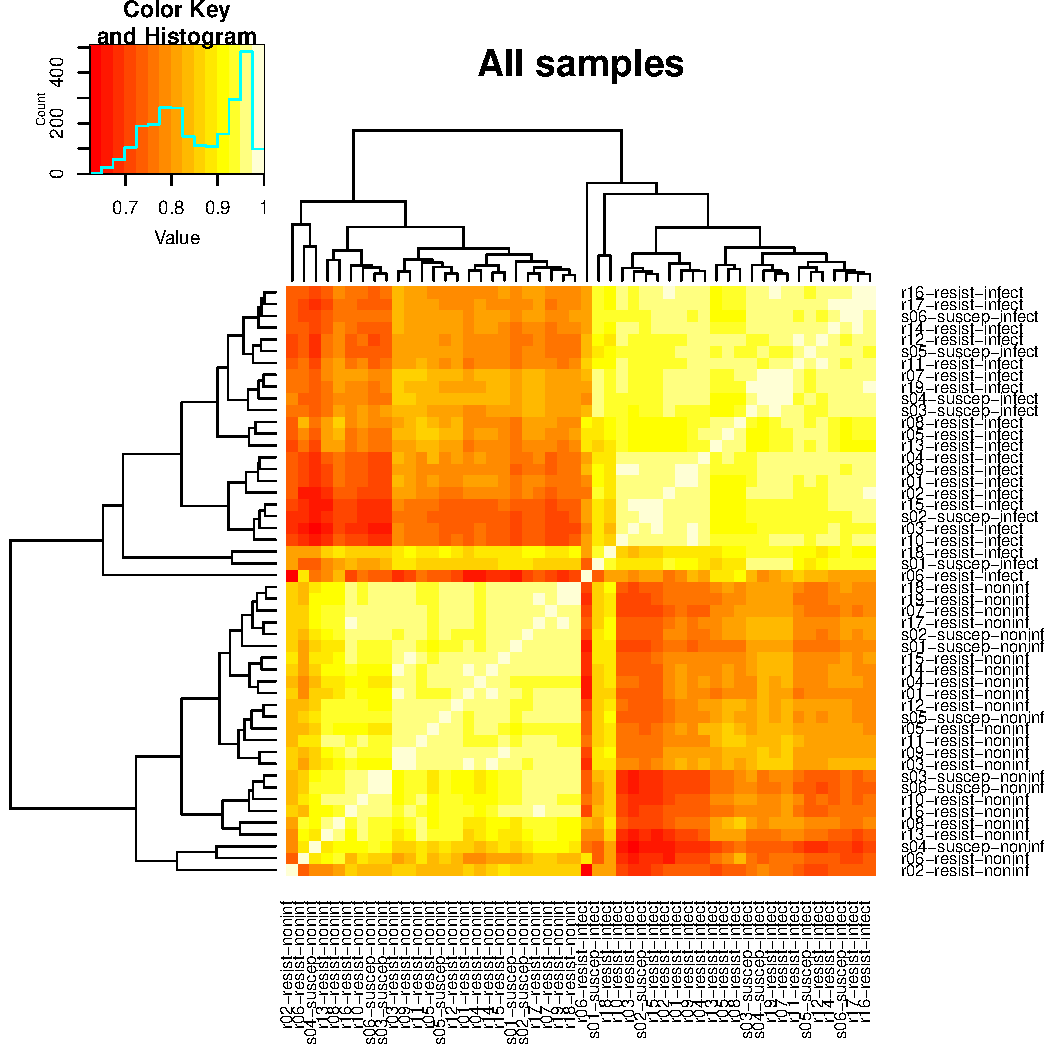
\includegraphics[width=\linewidth]{../figure/heatmap-all-samples.pdf}
\caption{
Heatmap of correlation matrix of samples. Each square represents the
Pearson correlation between the log\textsubscript{2} cpm expression
values of two samples. Red indicates a low correlation of zero and
white represents a high correlation of 1. The dendrogram displays the
results of hierarchical clustering with the complete linkage method.
The outliers of the non-infected samples are s04-suscept-noninf,
r02-resist-noninf, and r06-resist-noninf. The outliers of the infected
samples are s01-suscep-infect, r06-resist-infect, and
r18-resist-infect.
}
\label{fig:heat-all}
\end{figure}

\begin{figure}[ht]
\centering
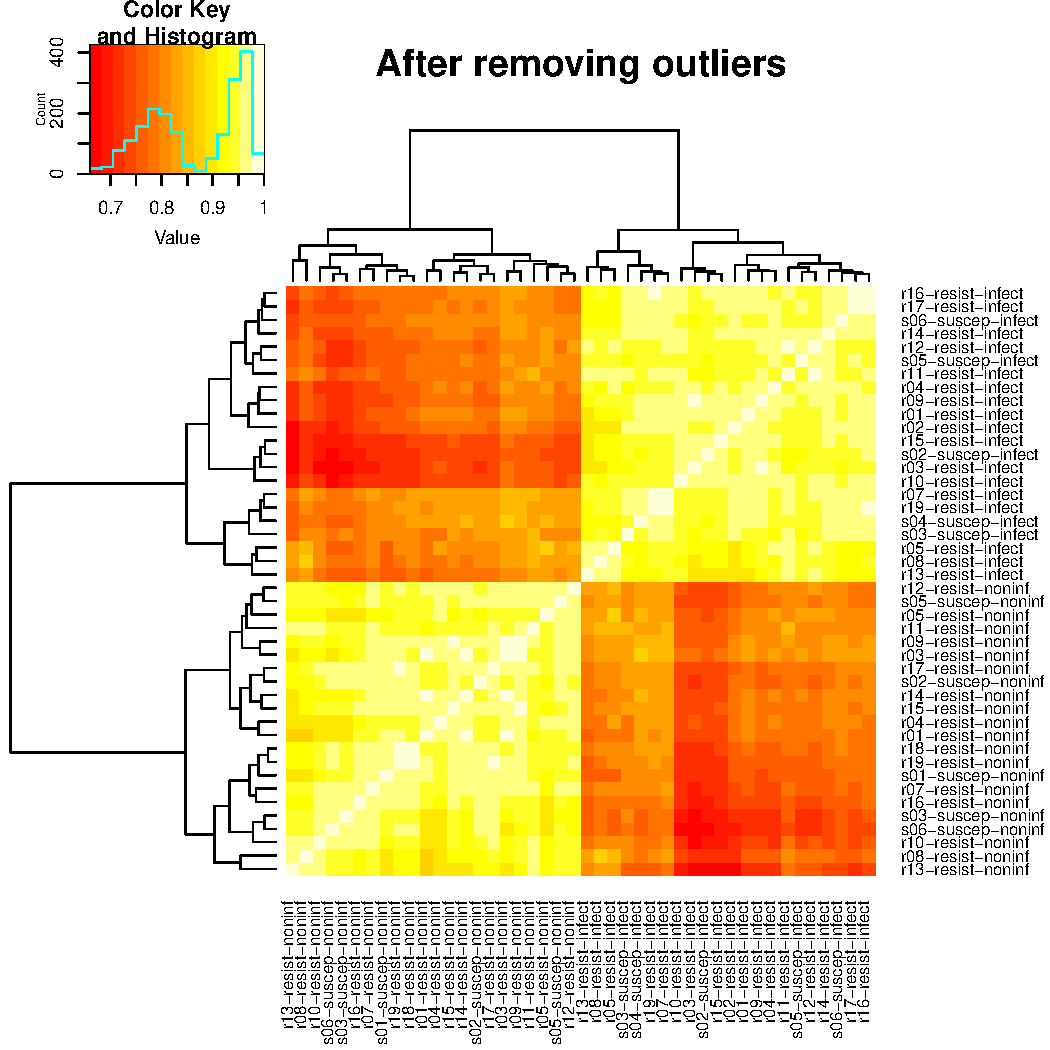
\includegraphics[width=\linewidth]{../figure/heatmap-no-outliers.pdf}
\caption{
Heatmap of correlation matrix after removing outliers. Each square
represents the Pearson correlation between the log\textsubscript{2}
cpm expression values of two samples. Red indicates a low correlation
of zero and white represents a high correlation of 1. The dendrogram
displays the results of hierarchical clustering with the complete
linkage method.
}
\label{fig:heat-filt}
\end{figure}


\begin{figure}[ht]
\centering
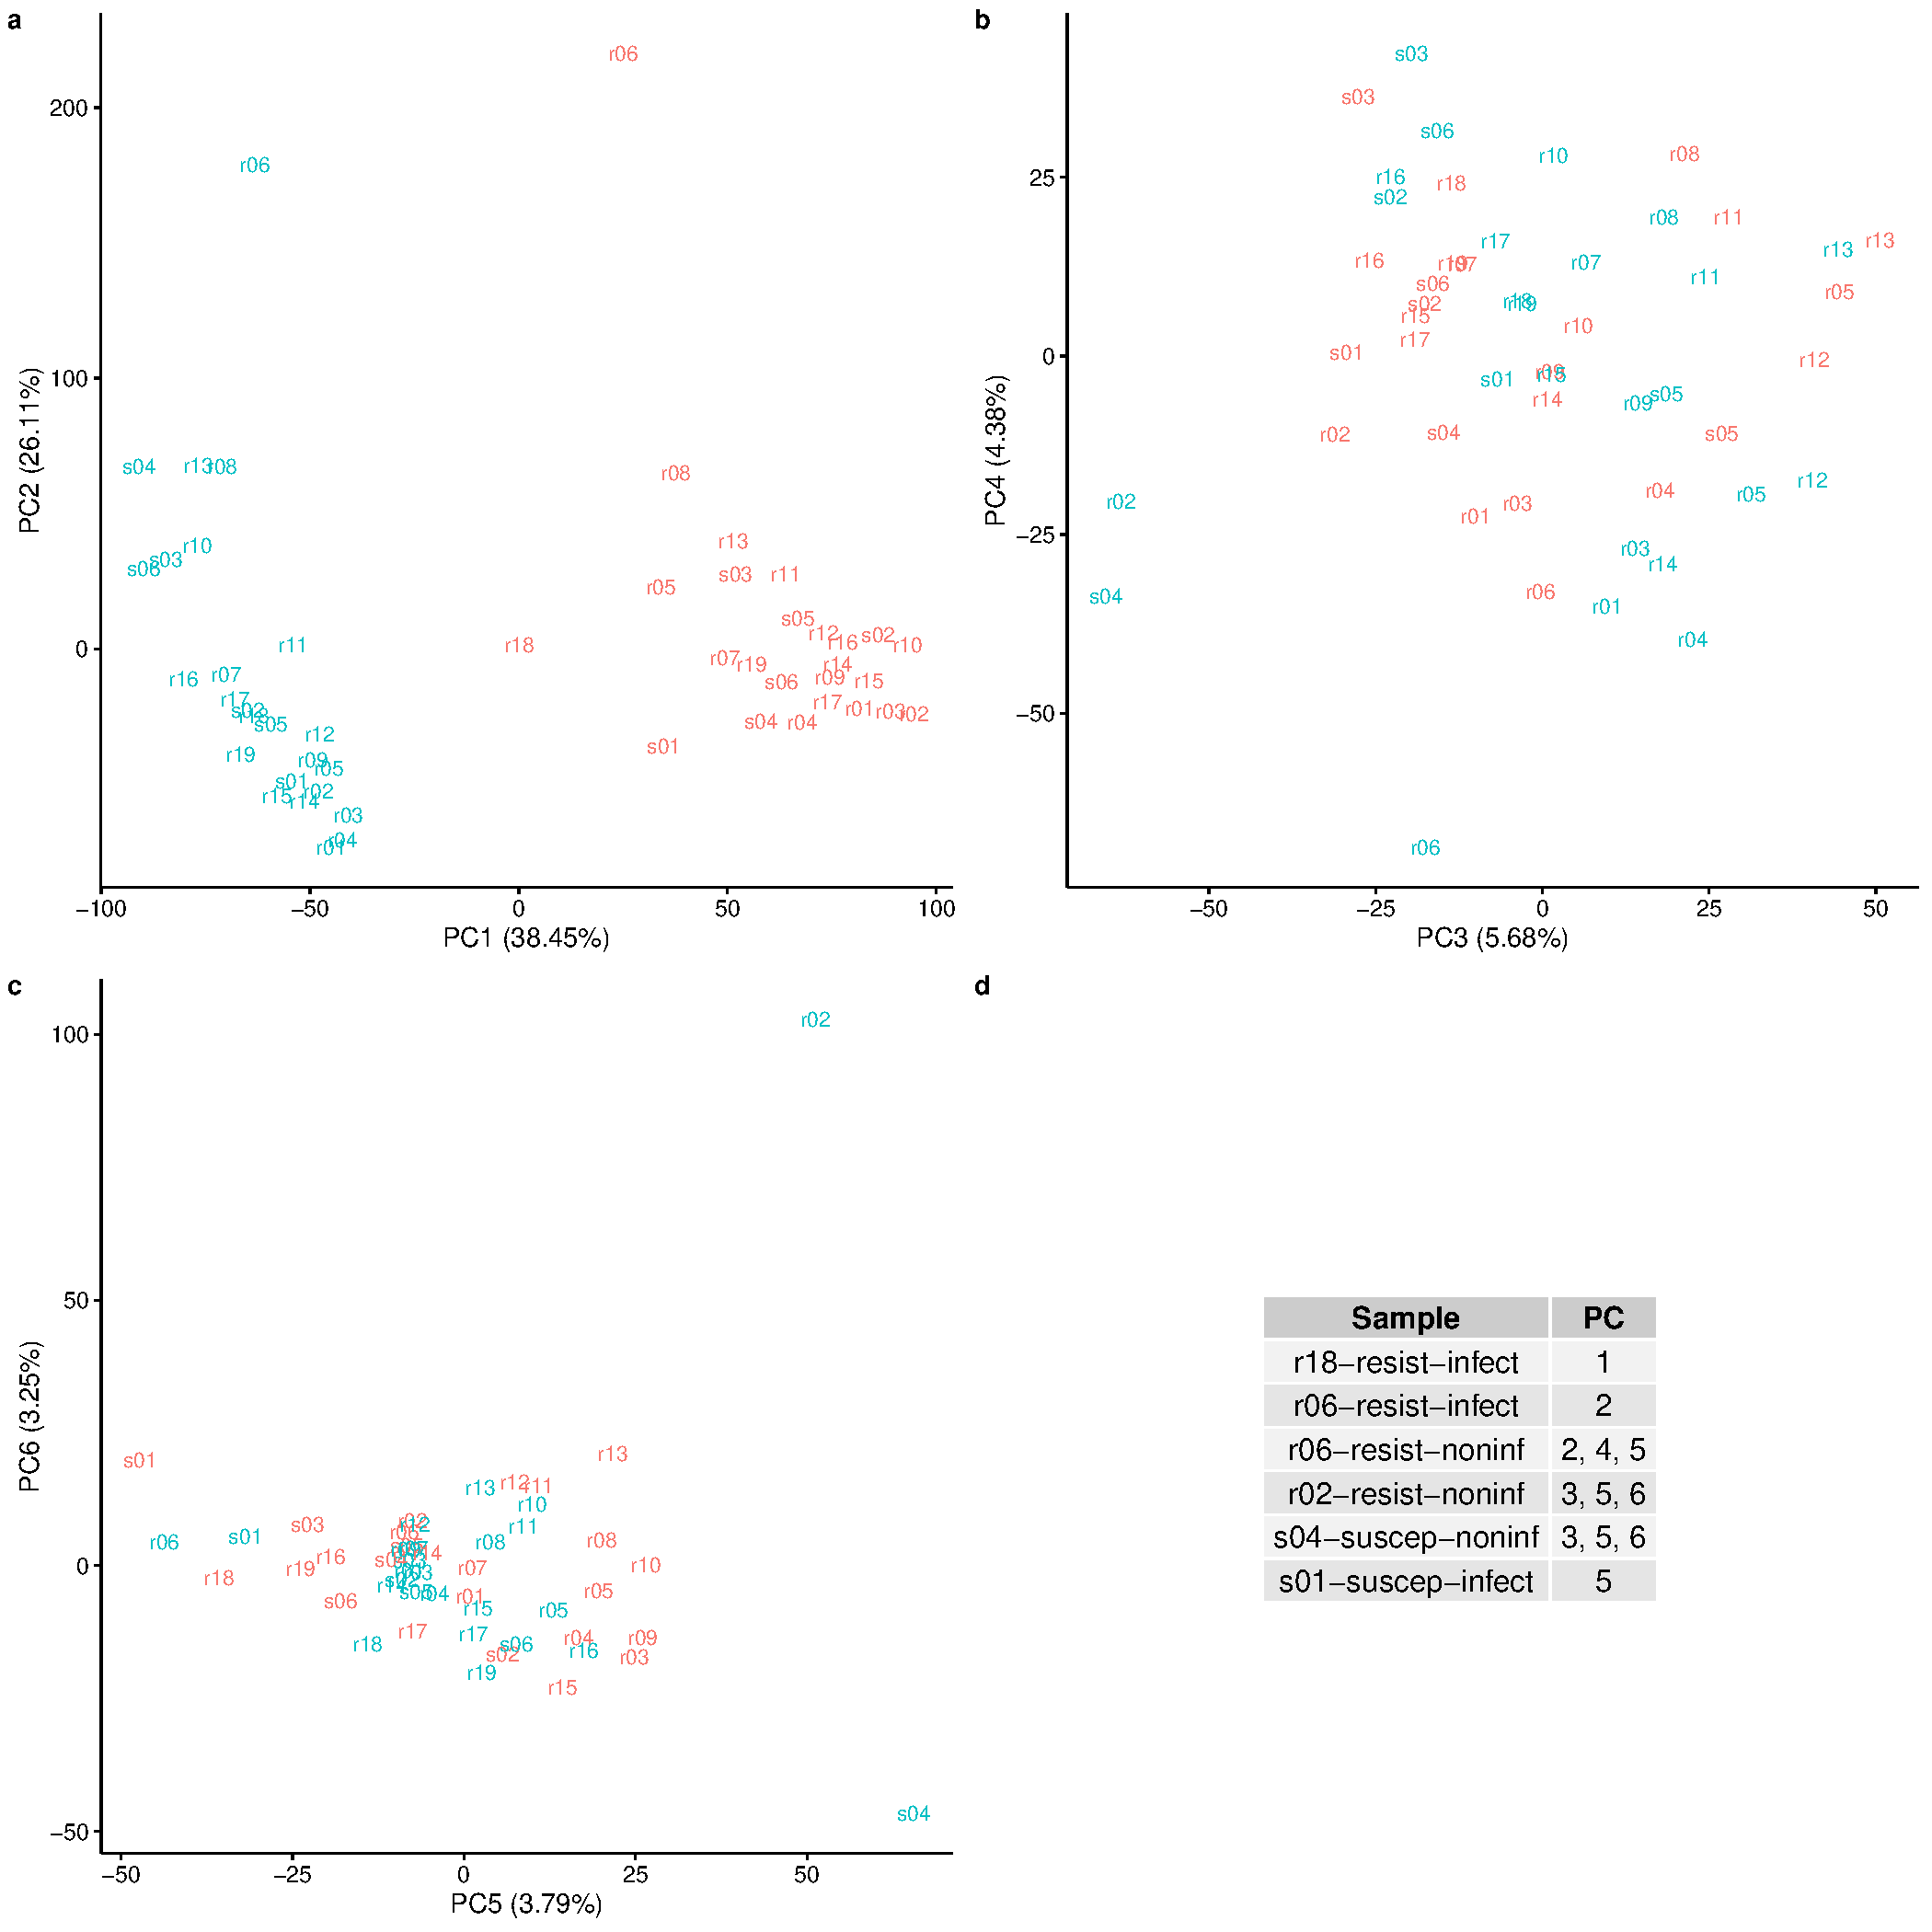
\includegraphics[width=\linewidth]{../figure/outliers.pdf}
\caption{
Principal components analysis (PCA) to identify outliers. (a) PC1
versus PC2, (b) PC3 versus PC4, and (c) PC5 versus PC6. Each sample is
represented by its 3-letter ID. “s” stands for susceptible and “r” for
resistant, and the text is colored on the basis of treatment status
(purple is non-infected; green is infected). The value in parentheses
in each axis is the percentage of total variation accounted for by
that PC. The outliers are listed in (d). These samples do not fall
within 2 standard deviations of the mean value of the PCs listed in
the right column. Note that a separate mean was calculated for the
non-infected and infected samples for PC1 only.
}
\label{fig:outliers}
\end{figure}


\begin{figure}[ht]
\centering
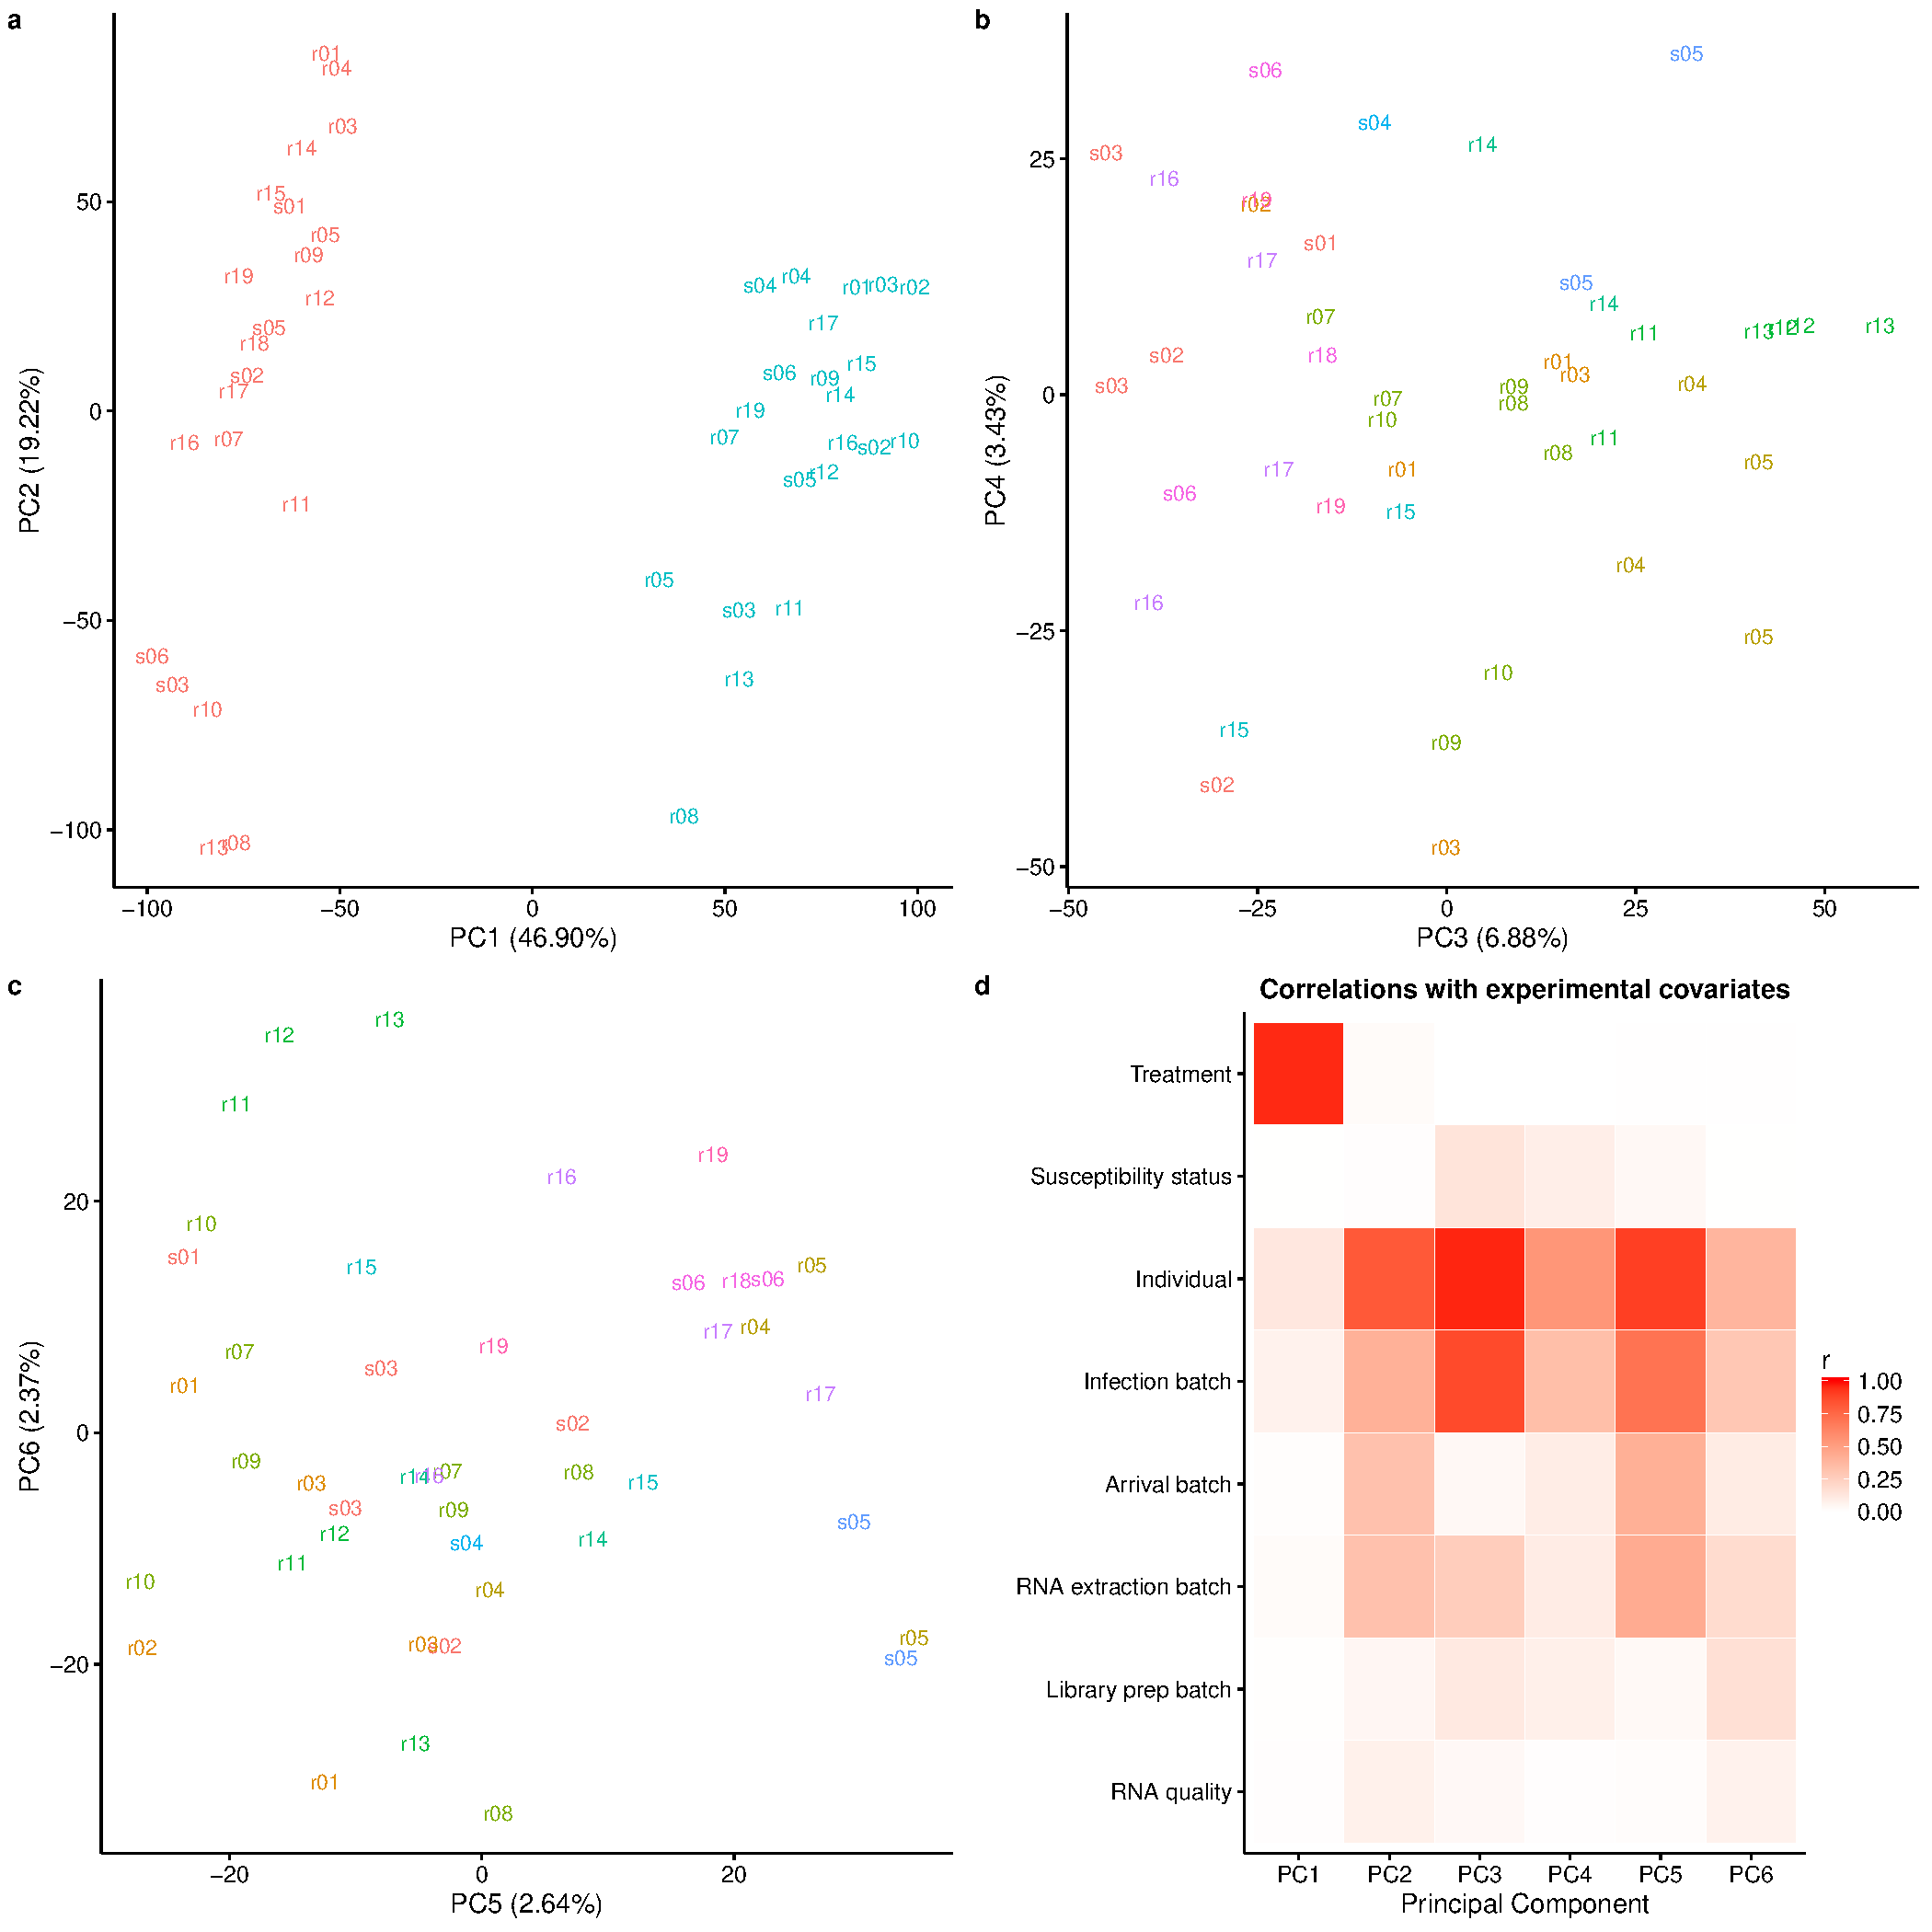
\includegraphics[width=\linewidth]{../figure/batch-pca.pdf}
\caption{
Check for technical batch effects using principal components analysis
(PCA). (a) PC1 versus PC2. The text labels are the individual
identifiers. Purple indicates non-infected samples and green indicates
infected. (b) PC3 versus PC4. The colors indicate the different
infection batches. (c) PC5 versus PC6. The colors indicate the
different infection batches. (d) The Pearson correlation of PCs 1-6
with each of the recorded biological and technical covariates. The
correlations vary from 0 (white) to 1 (red).
}
\label{fig:batch}
\end{figure}

\begin{figure}[ht]
\centering
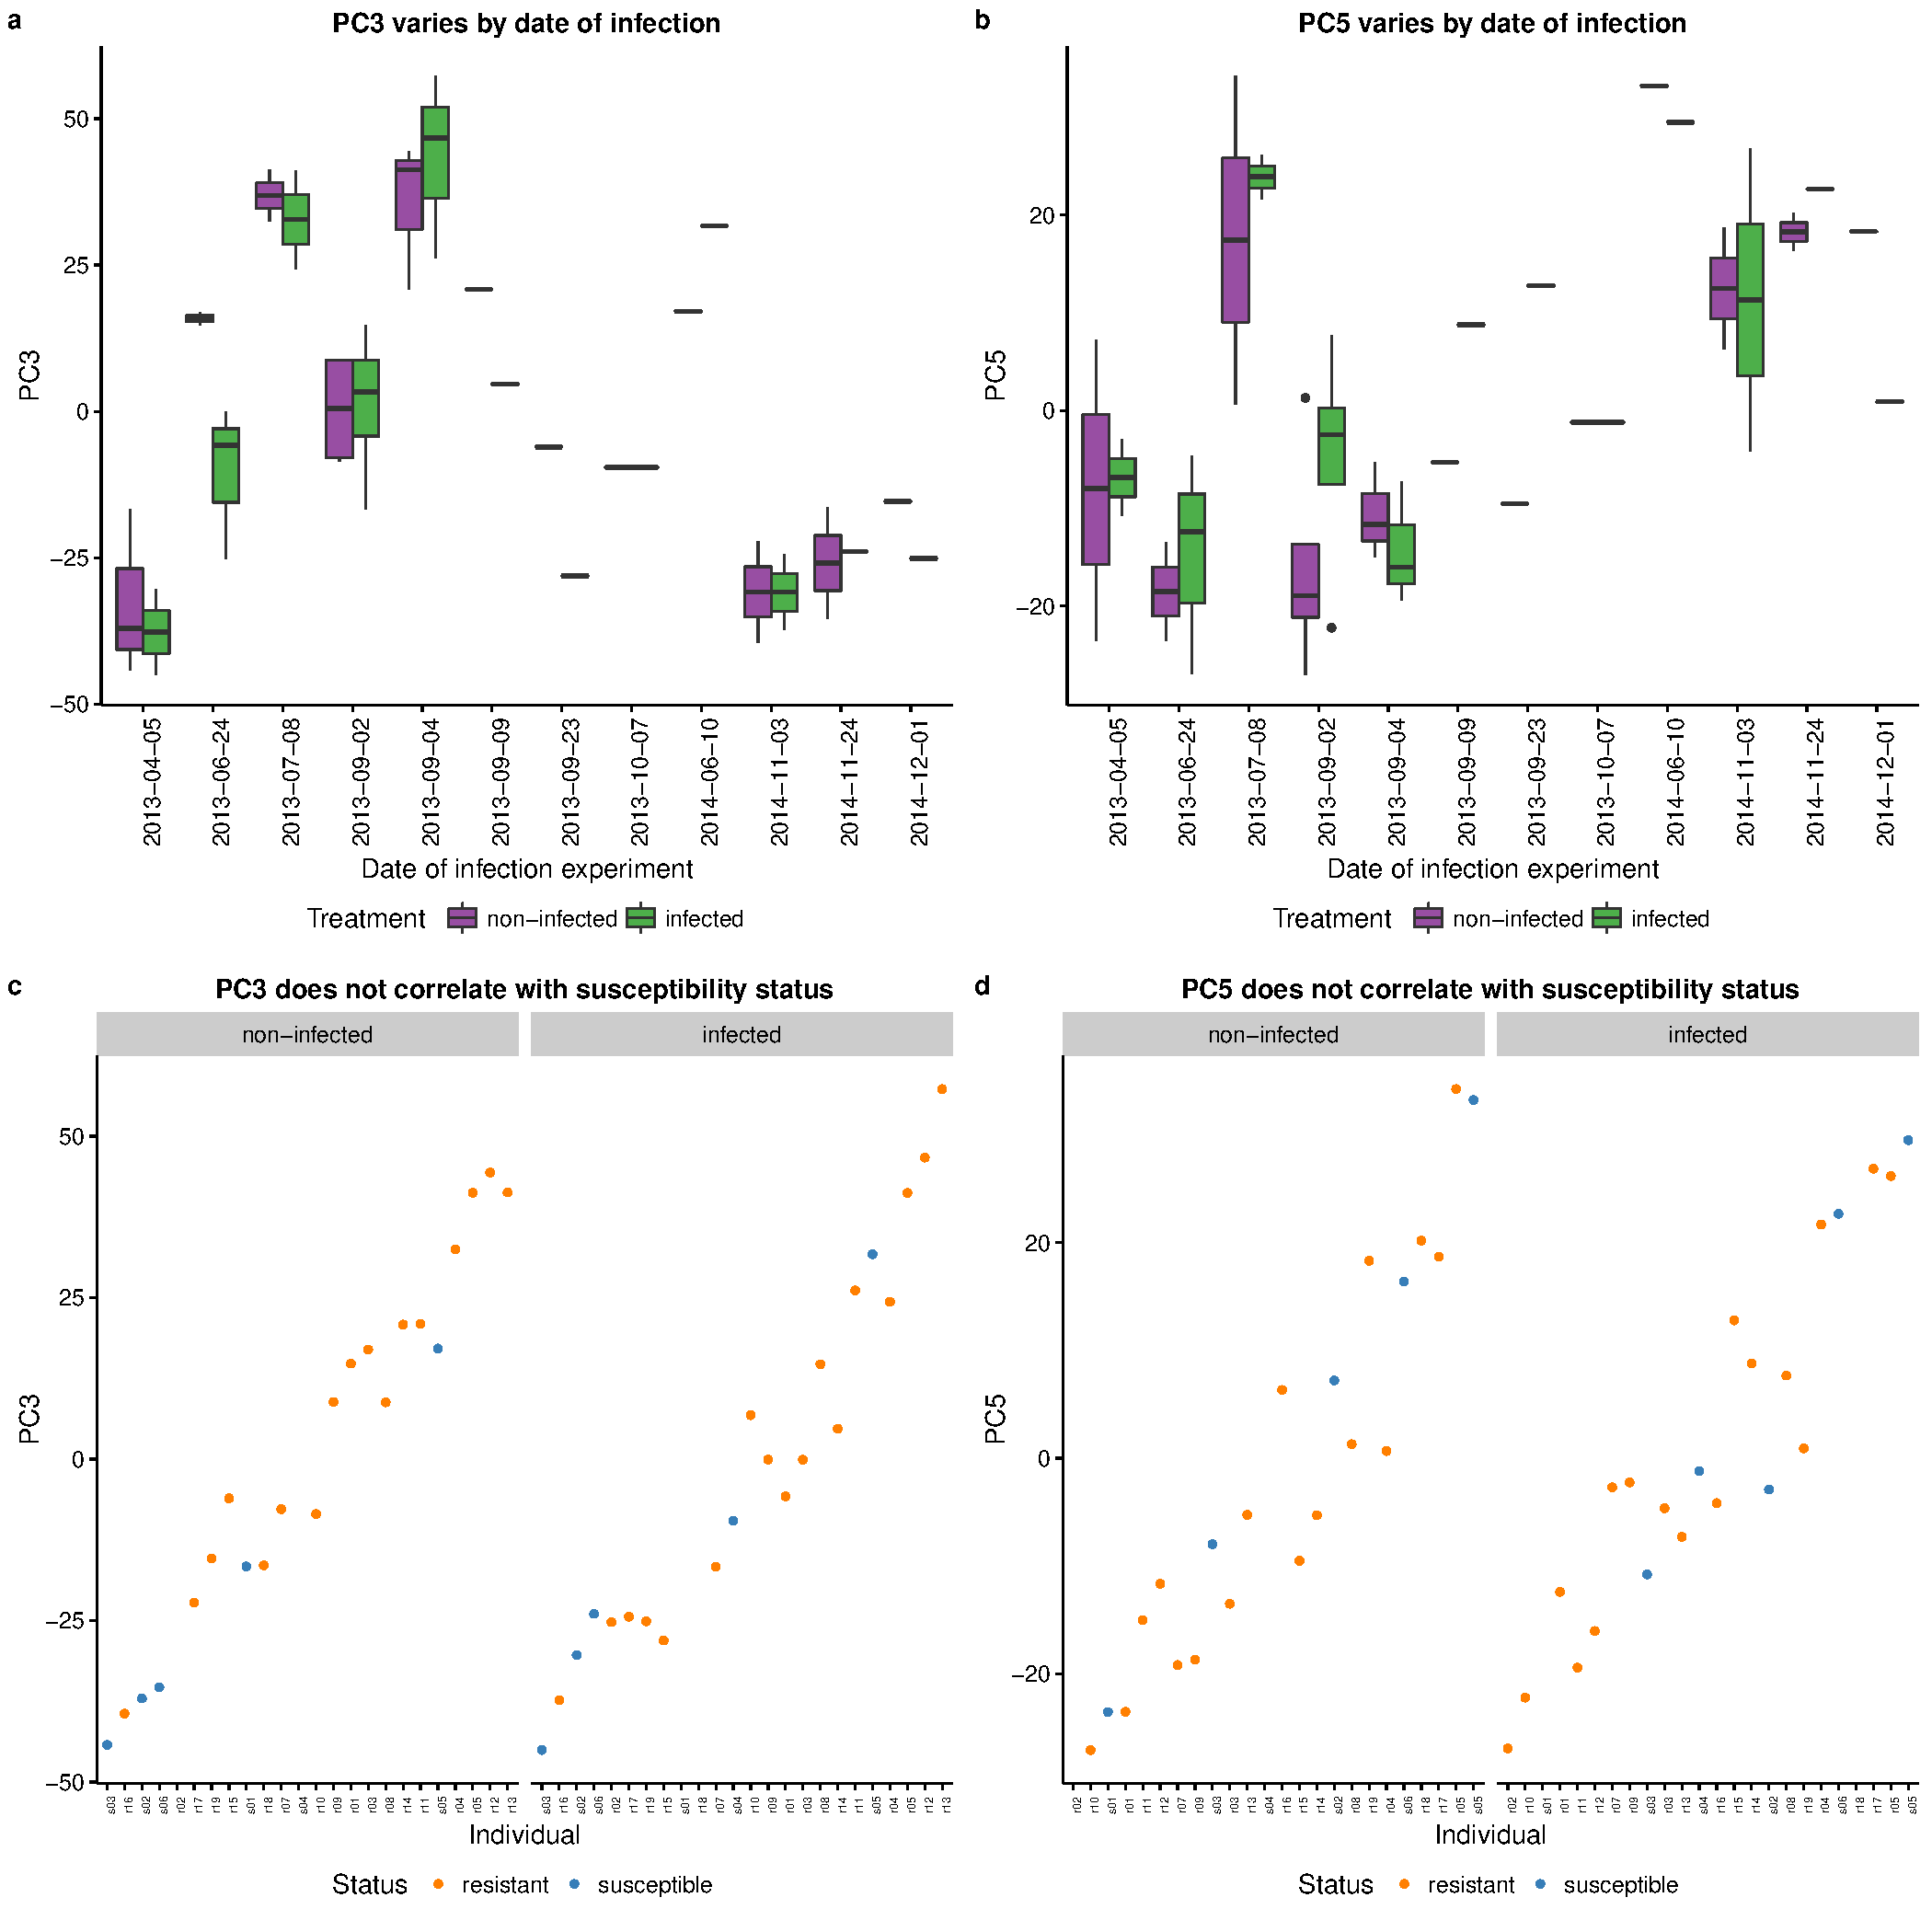
\includegraphics[width=\linewidth]{../figure/batch-infection.pdf}
\caption{
Check for confounding effect of infection batch. PC3 (a) and PC5 (b)
varied by the date of infection. Non-infected samples are in purple
and infected samples in green. Importantly, however, this technical
variation arising from infection batch did not correlate with the
susceptibility status of the individuals (c and d). Resistant
individuals are in orange and susceptible individuals in blue.
}
\label{fig:infection}
\end{figure}

\begin{figure}[ht]
\centering
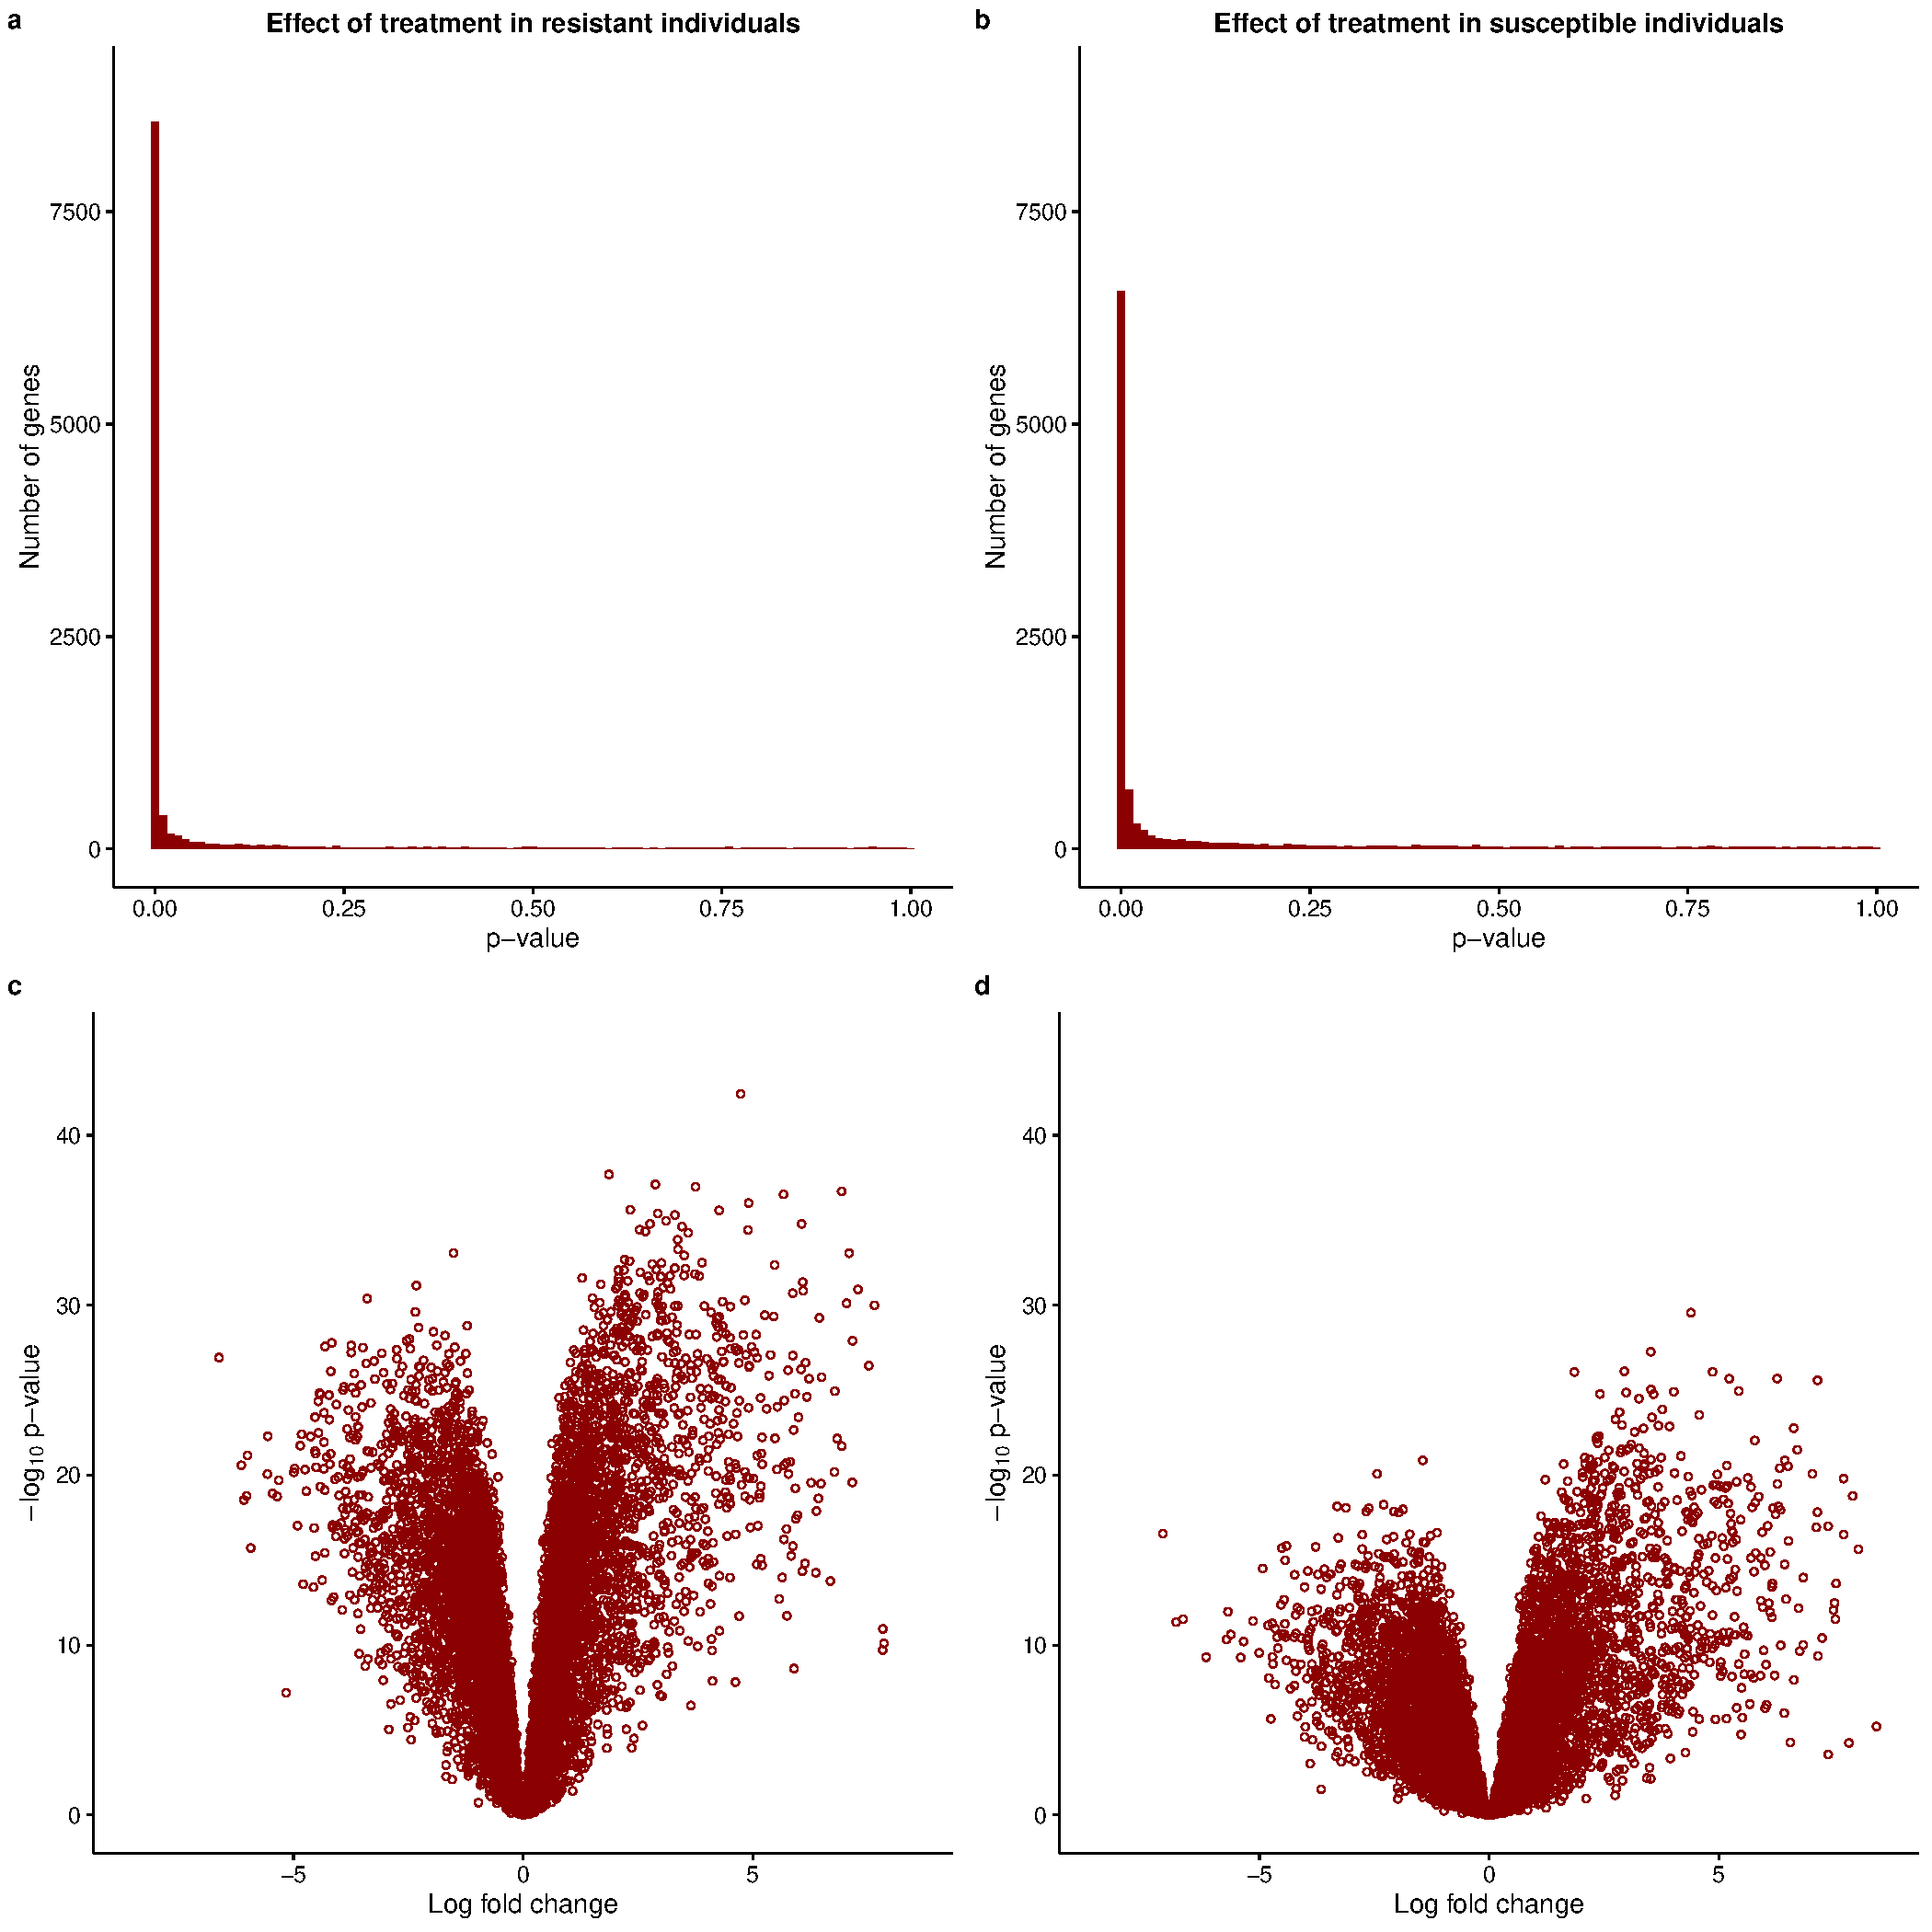
\includegraphics[width=\linewidth]{../figure/limma-supp.pdf}
\caption{
Effect of treatment with MTB. The top panel contains the distribution
of unadjusted p-values after testing for differential expression
between the non-infected and infected states in (a) resistant and (b)
susceptible individuals. The bottom panel contains the corresponding
volcano plots for the (c) resistant and (d) susceptible individuals.
The x-axis is the log fold change in gene expression level between
susceptible and resistant individuals and the y-axis is the
–log\textsubscript{10} p-value. Red indicates genes which are
significant differentially expressed with a q-value less than 10\%.
Because of the extremely skewed p-value distribution, all genes are
significantly differentially expressed at this false discovery rate.
}
\label{fig:limma-supp}
\end{figure}

\begin{figure}[ht]
\centering
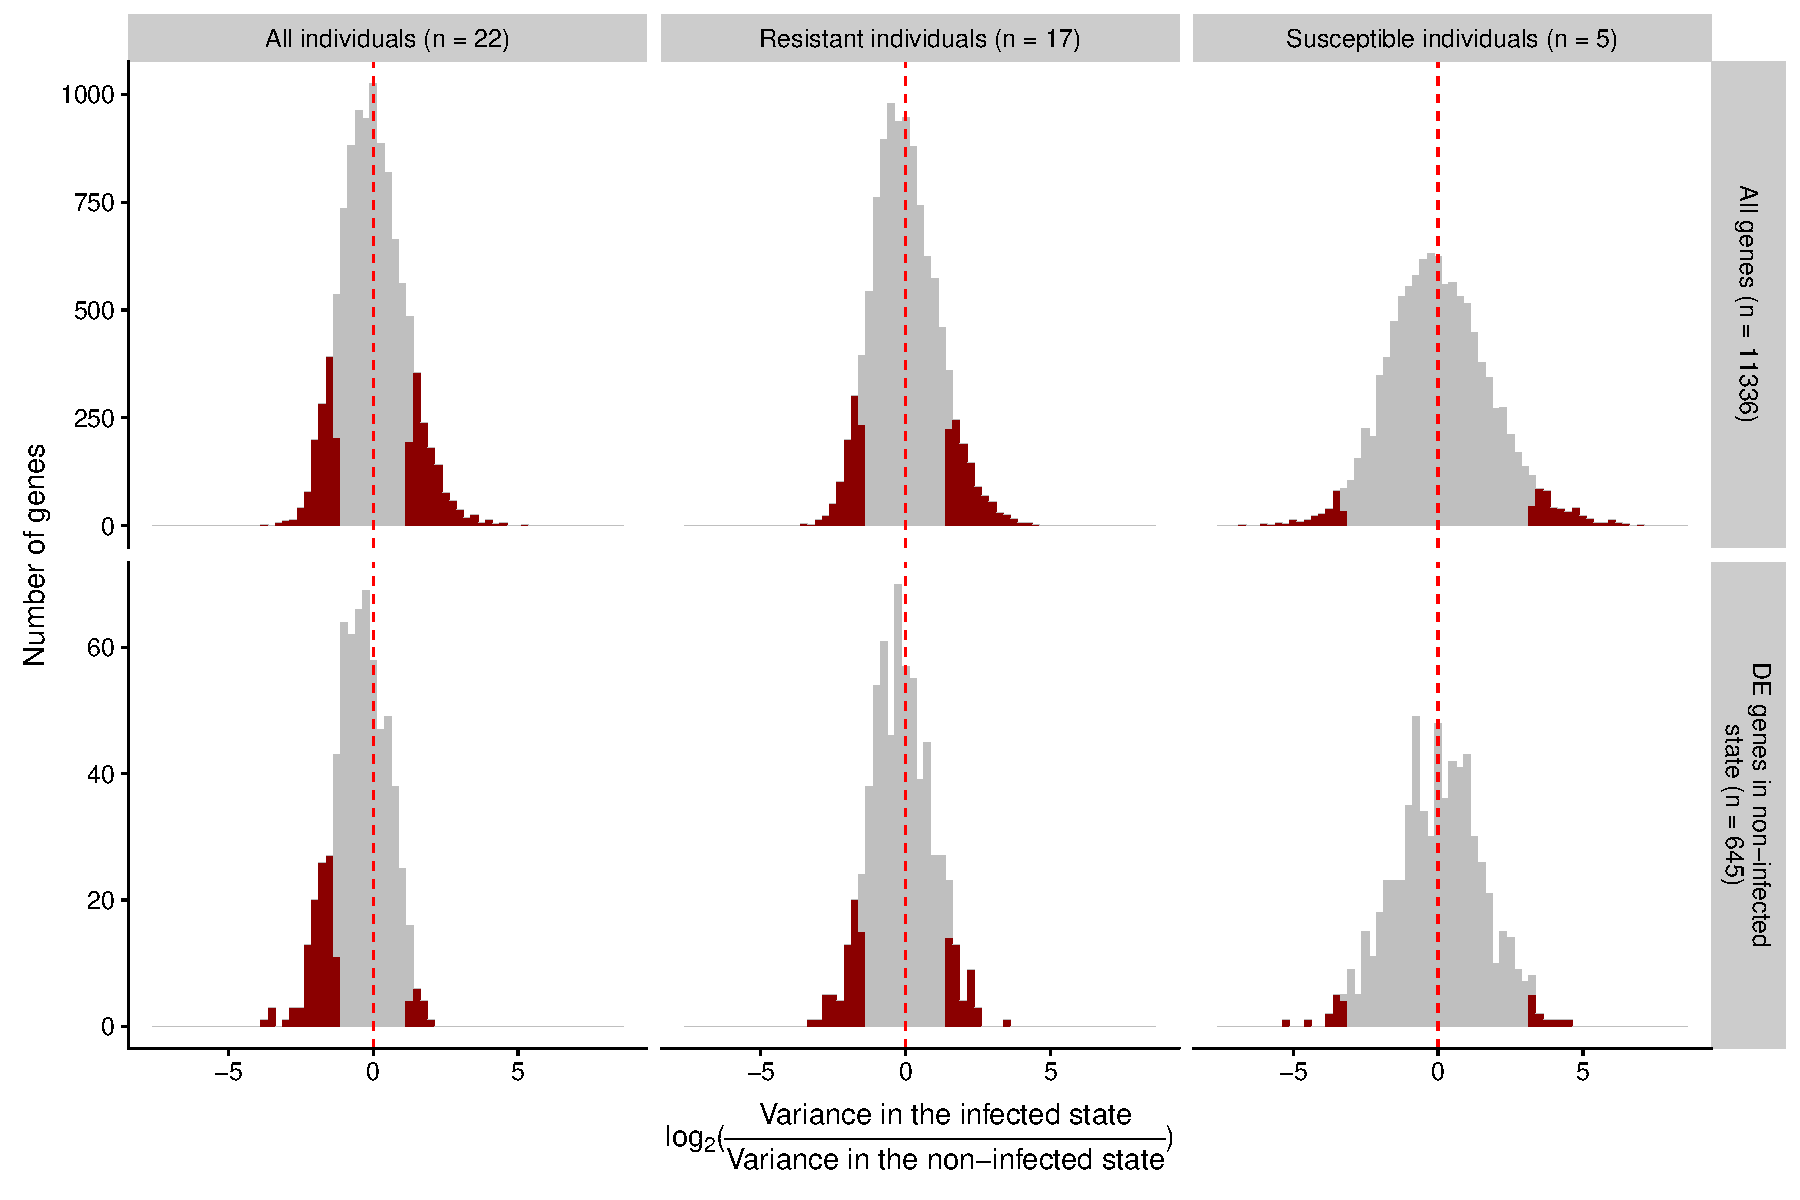
\includegraphics[width=\linewidth]{../figure/variance.pdf}
\caption{
Check for systematic differences in gene expression variance between
the infected and non-infected states. We identified DE genes between
susceptible and resistant individuals in the non-infected but not the
infected state. Could this be a statistical artifact due to an overall
increase in gene expression variance upon infection thus reducing
power to detect DE genes? No, because we did not observe an overall
increase in gene expression variance in the infected state. The
histograms show the distribution of the
log\textsubscript{2}-transformed ratio of the gene expression variance
in the infected state to the variance in the non-infected state. If
there was an overall increase in variance, the distributions should be
shifted towards the right, but instead they are all symmetrical. The
top row shows the results for the 10,691 genes which were not
differentially expressed between susceptible and resistant individuals
in the non-infected state, and the bottom row shows the results for
the 645 genes which were. The left column shows the results for all 22
individuals in the study, the middle column for the 17 resistant
individuals, and the right column for the 5 susceptible individuals
(note that the right column has the widest spread because of this
small sample size). Highlighted in red are genes which had a \emph{P}
\textless \, 0.05 from an F test comparing the two variances. The
number of genes with a significant increase or decrease in variance
was also mostly symmetrical (decrease vs. increase starting at top
left panel and proceeding clockwise: 1,232 vs. 1,362; 934 vs. 1,118;
275 vs. 455; 13 vs. 11; 64 vs. 44; 108 vs. 15).
}
\label{fig:variance}
\end{figure}


\begin{figure}[ht]
\centering
\includegraphics[width=6in]{../figure/gwas-figures.pdf}
\caption{
Comparison of differential expression and GWAS results. In each
subplot, the y-axis is the fold enrichment (y-axis) of genes assigned
a SNP with p-value less than 0.05 from the GWAS. The x-axis is bins of
genes with increasingly stringent effect size cutoffs of the absolute
log fold change for the different expression contrast. The effect size
cutoffs were chosen such that each bin from left to right contained
approximately 25 fewer genes. The red line is the results from the
actual data. The grey lines are the results from 100 permutations. The
dashed blue line at y=1 is the null expectation. The rows correspond
to the 5 GWAS studies: Russia \cite{Curtis2015}, The Gambia
\cite{Thye2010}, Ghana \cite{Thye2010}, Uganda and Tanzania
\cite{Sobota2016}, and height in individuals of European ancestry
\cite{LangoAllen2010}. The columns correspond to the 4 differential
expression contrasts: resistant vs. susceptible individuals in the
non-infected state (status\_ni), resistant vs. susceptible individuals
in the infected state (status\_ii), effect of treatment in resistant
individuals (treat\_resist), and effect of treatment in susceptible
individuals (treat\_suscep). The x-axis slightly varies based on the
number of genes that were able to be assigned a nearby SNP for each
GWAS, and thus is consistent only within each study (i.e. row,
although the exact tick labels in each plot slightly vary based on R’s
rules for annotating axes). The y-axis is set separately for each plot
based on the minimum and maximum fold enrichment values for that
particular analysis.
}
\label{fig:gwas-supp}
\end{figure}

\begin{figure}[ht]
\centering
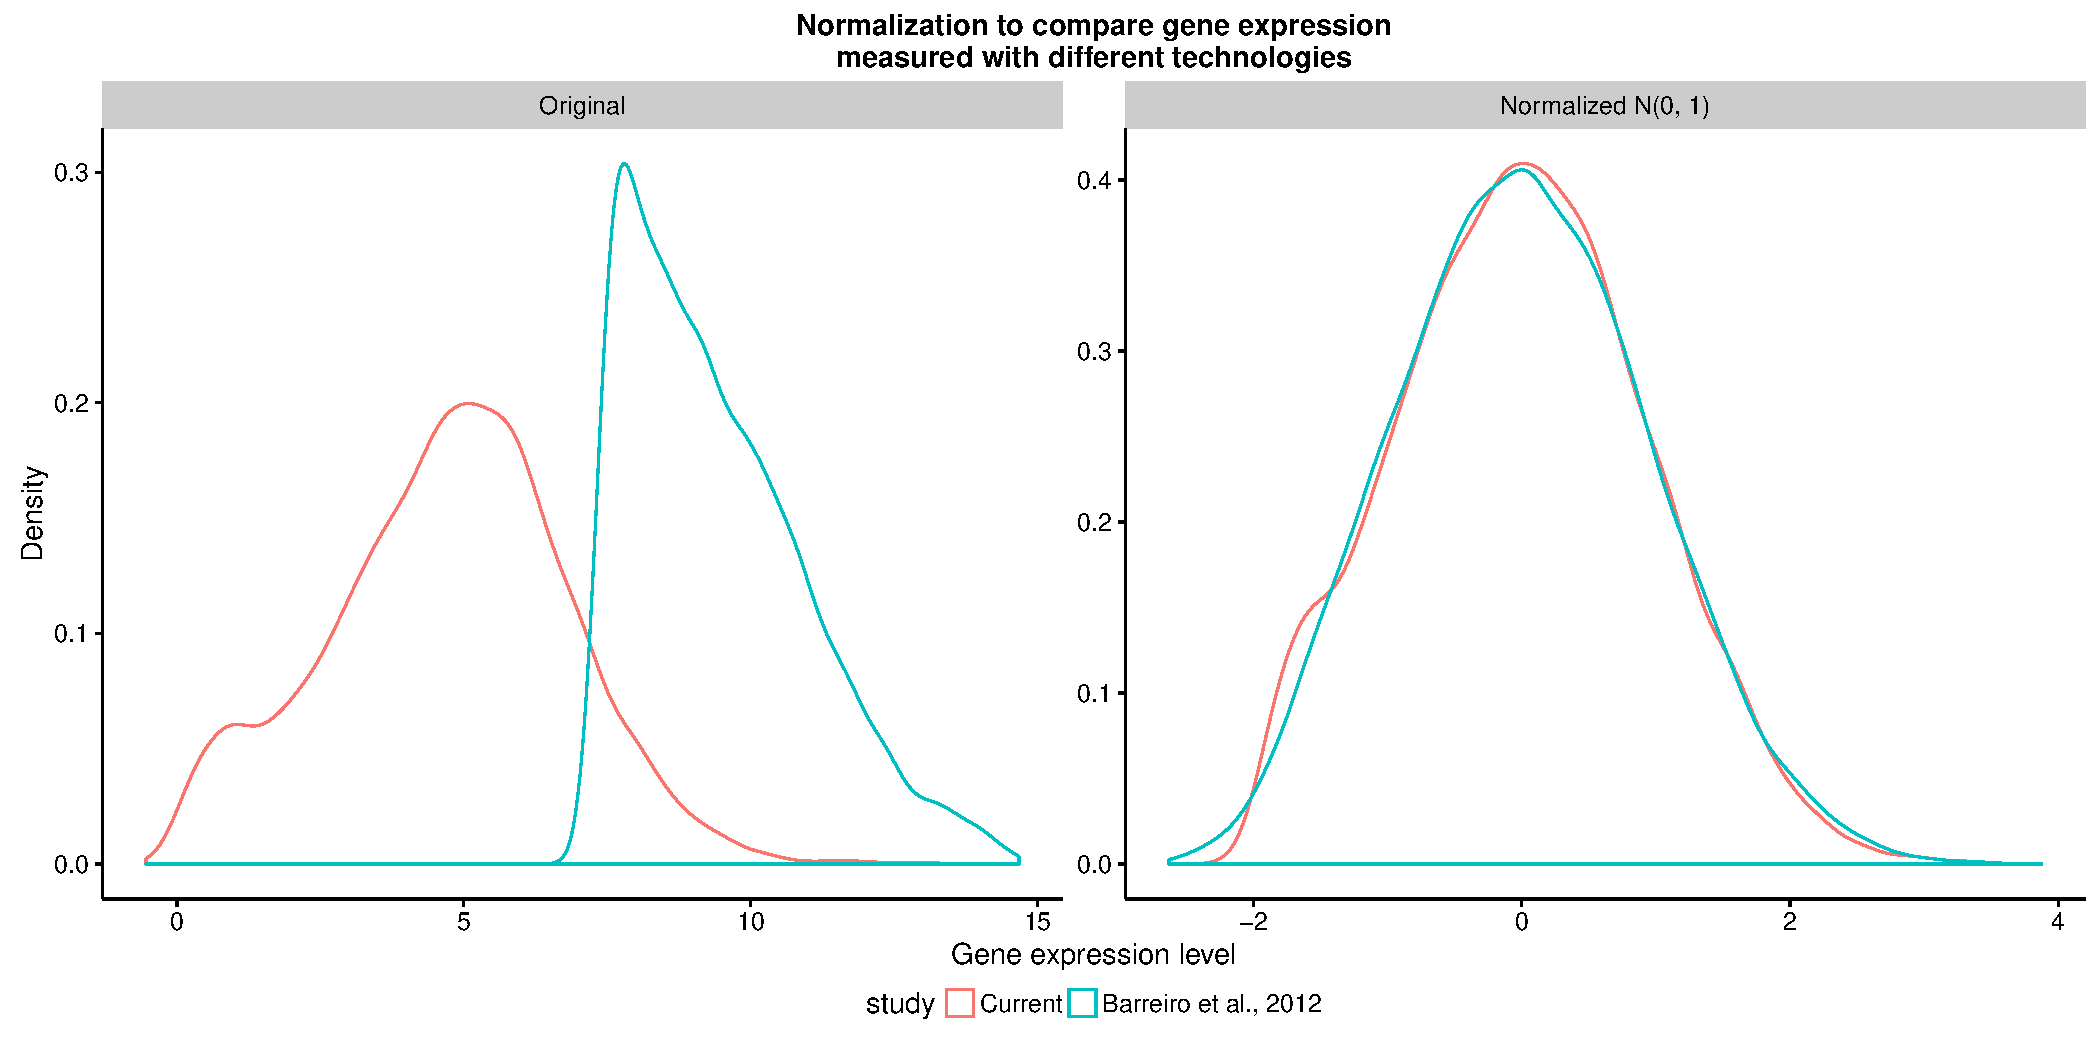
\includegraphics[width=\linewidth]{../figure/combined-distributions.pdf}
\caption{
Normalizing gene expression distributions. (left) The distribution of
the median log2 cpm of the RNA-seq data from the current study in red
compared to the distribution of the median gene expression levels of
the microarray data from Barreiro et al., 2012 \cite{Barreiro2012} in
blue. (right) The distributions of the same data sets after
normalizing each sample to a standard normal distribution.
}
\label{fig:combined-dist}
\end{figure}

\begin{figure}[ht]
\centering
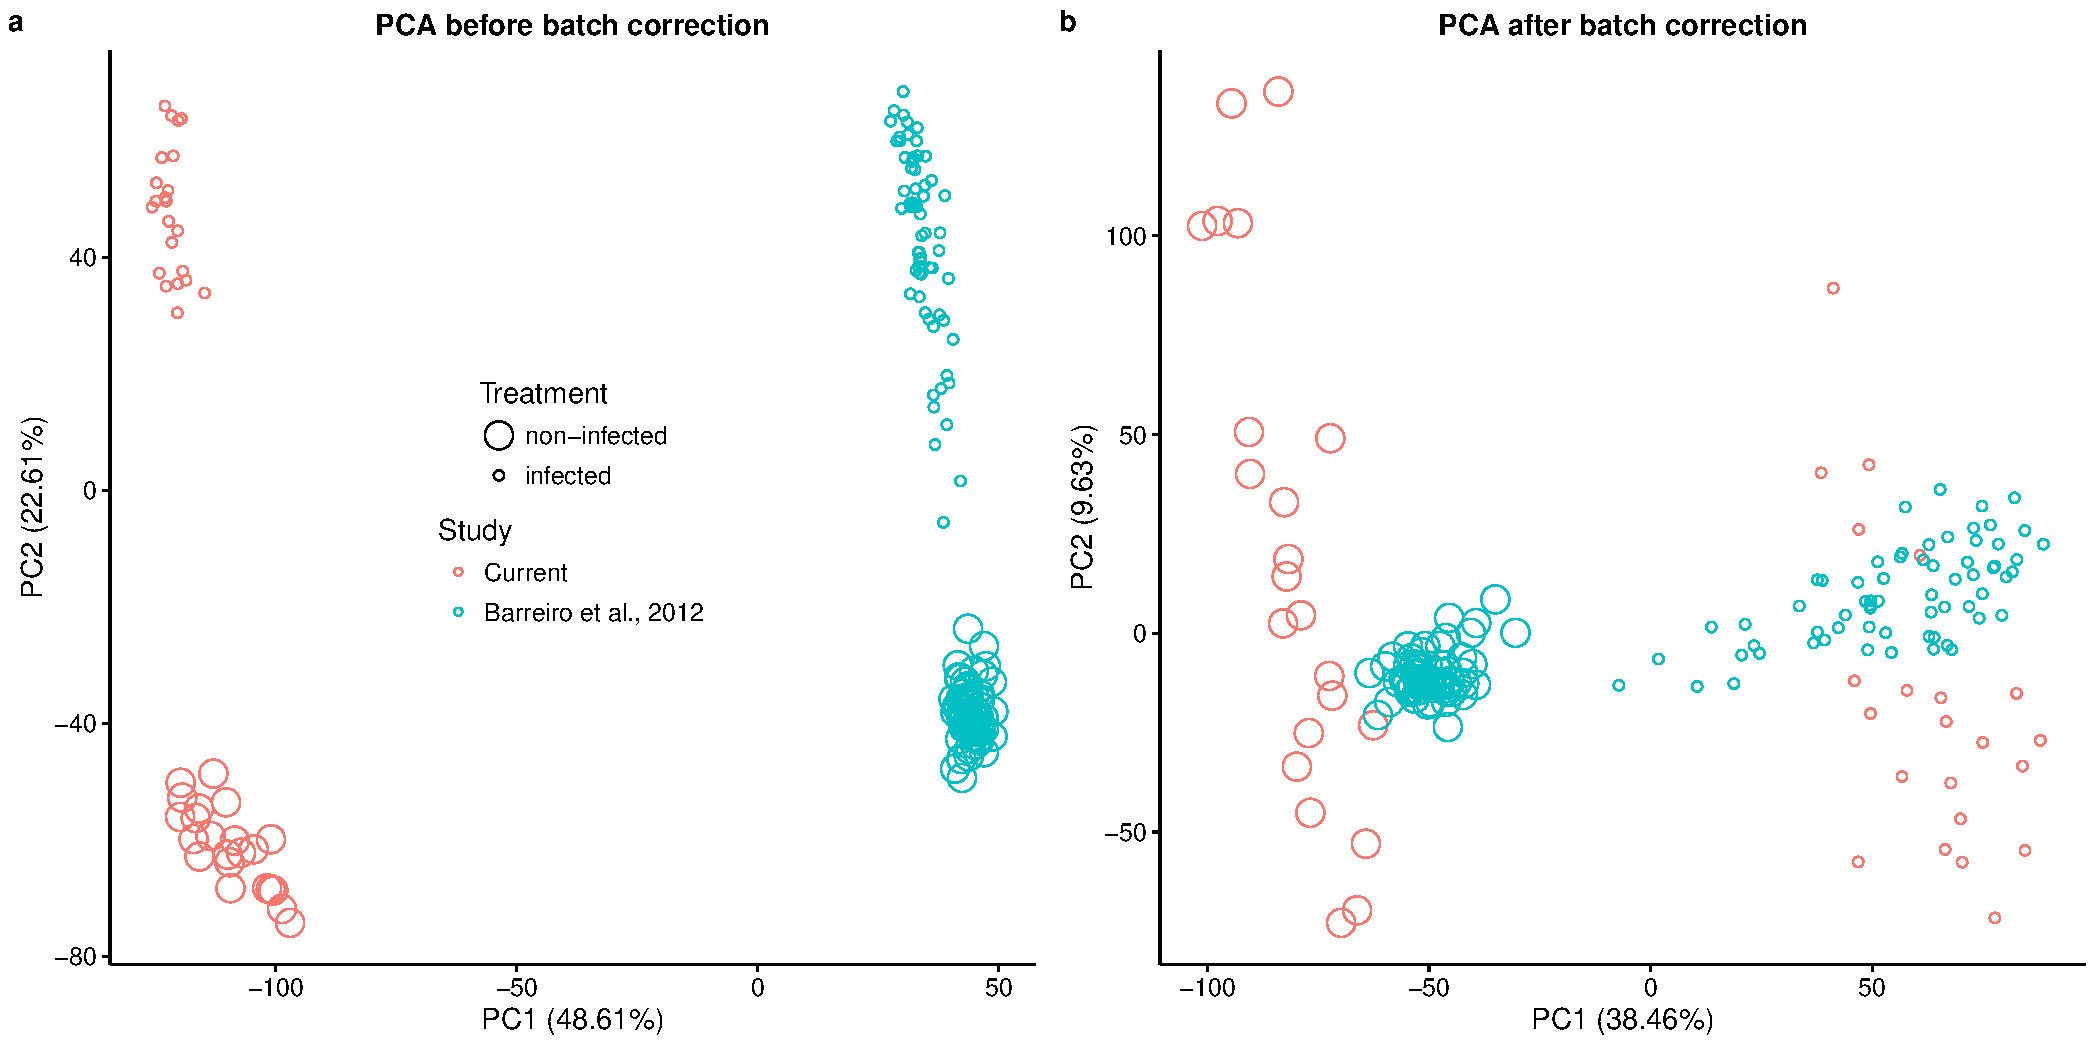
\includegraphics[width=\linewidth]{../figure/combined-pca.pdf}
\caption{
Principal components analysis (PCA) of combined data sets. (a) PC1
versus PC2 of the combined data set of the RNA-seq data from the
current study (red) and the microarray data from Barreiro et al., 2012
\cite{Barreiro2012} (blue). The large circles are non-infected
samples, and the small circles are infected samples. The value in
parentheses is the percentage of the total variation accounted for by
that PC. (b) The same data after regressing the original PC1 in (a).
}
\label{fig:combined-pca}
\end{figure}

\begin{figure}[ht]
\centering
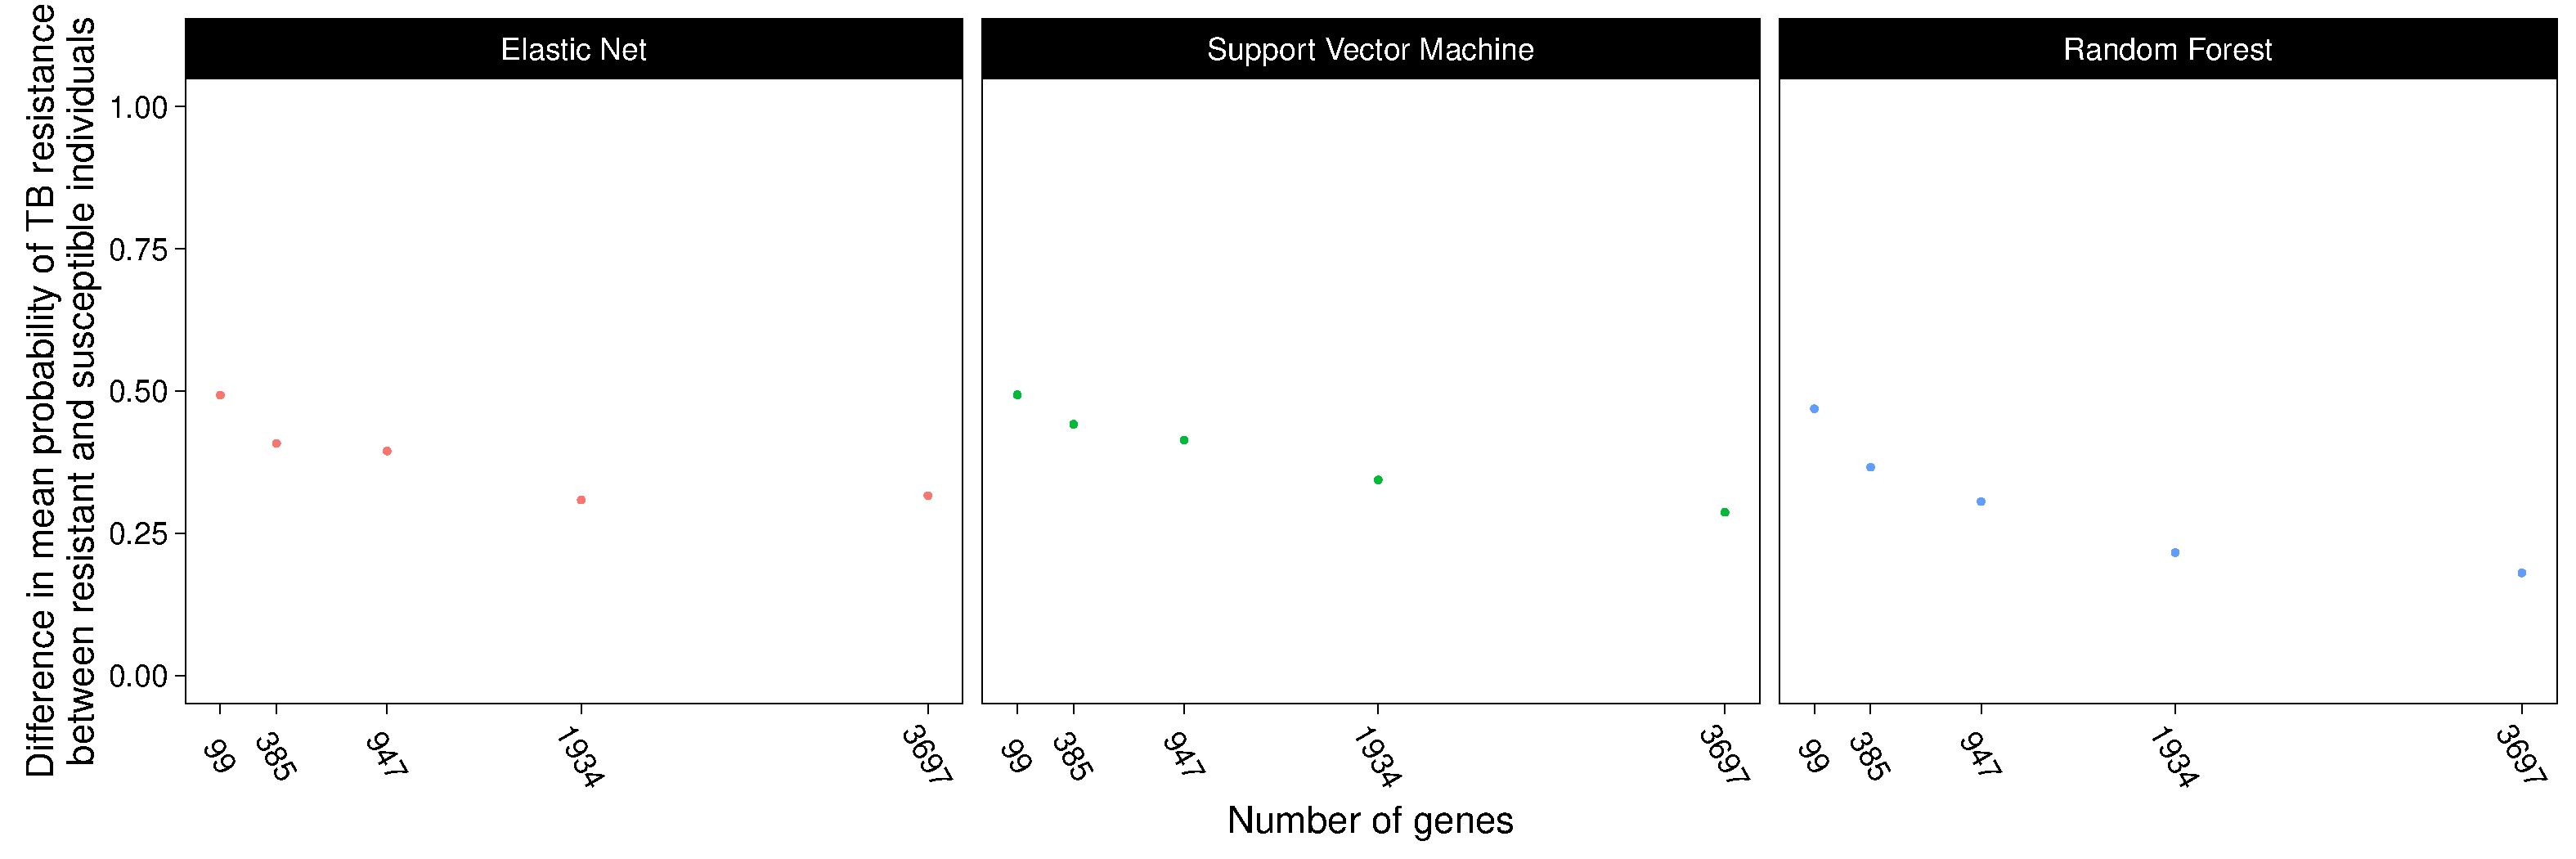
\includegraphics[width=\linewidth]{../figure/classifier-compare.pdf}
\caption{
Comparing the classification results of different methods and number
of input genes. We compared 3 different machine learning methods
(elastic net, support vector machine, random forest) and used 5
different sets of input genes. The input genes (x-axis) were obtained
by varying the q-value cutoff for differential expression between
susceptible and resistant individuals in the non-infected state from
5\% to 25\%. The evaluation metric (y-axis) was the difference of the
mean assigned probability of being TB resistant between the known
resistant and susceptible individuals in the current study.
}
\label{fig:class-compare}
\end{figure}

\begin{figure}[ht]
\centering
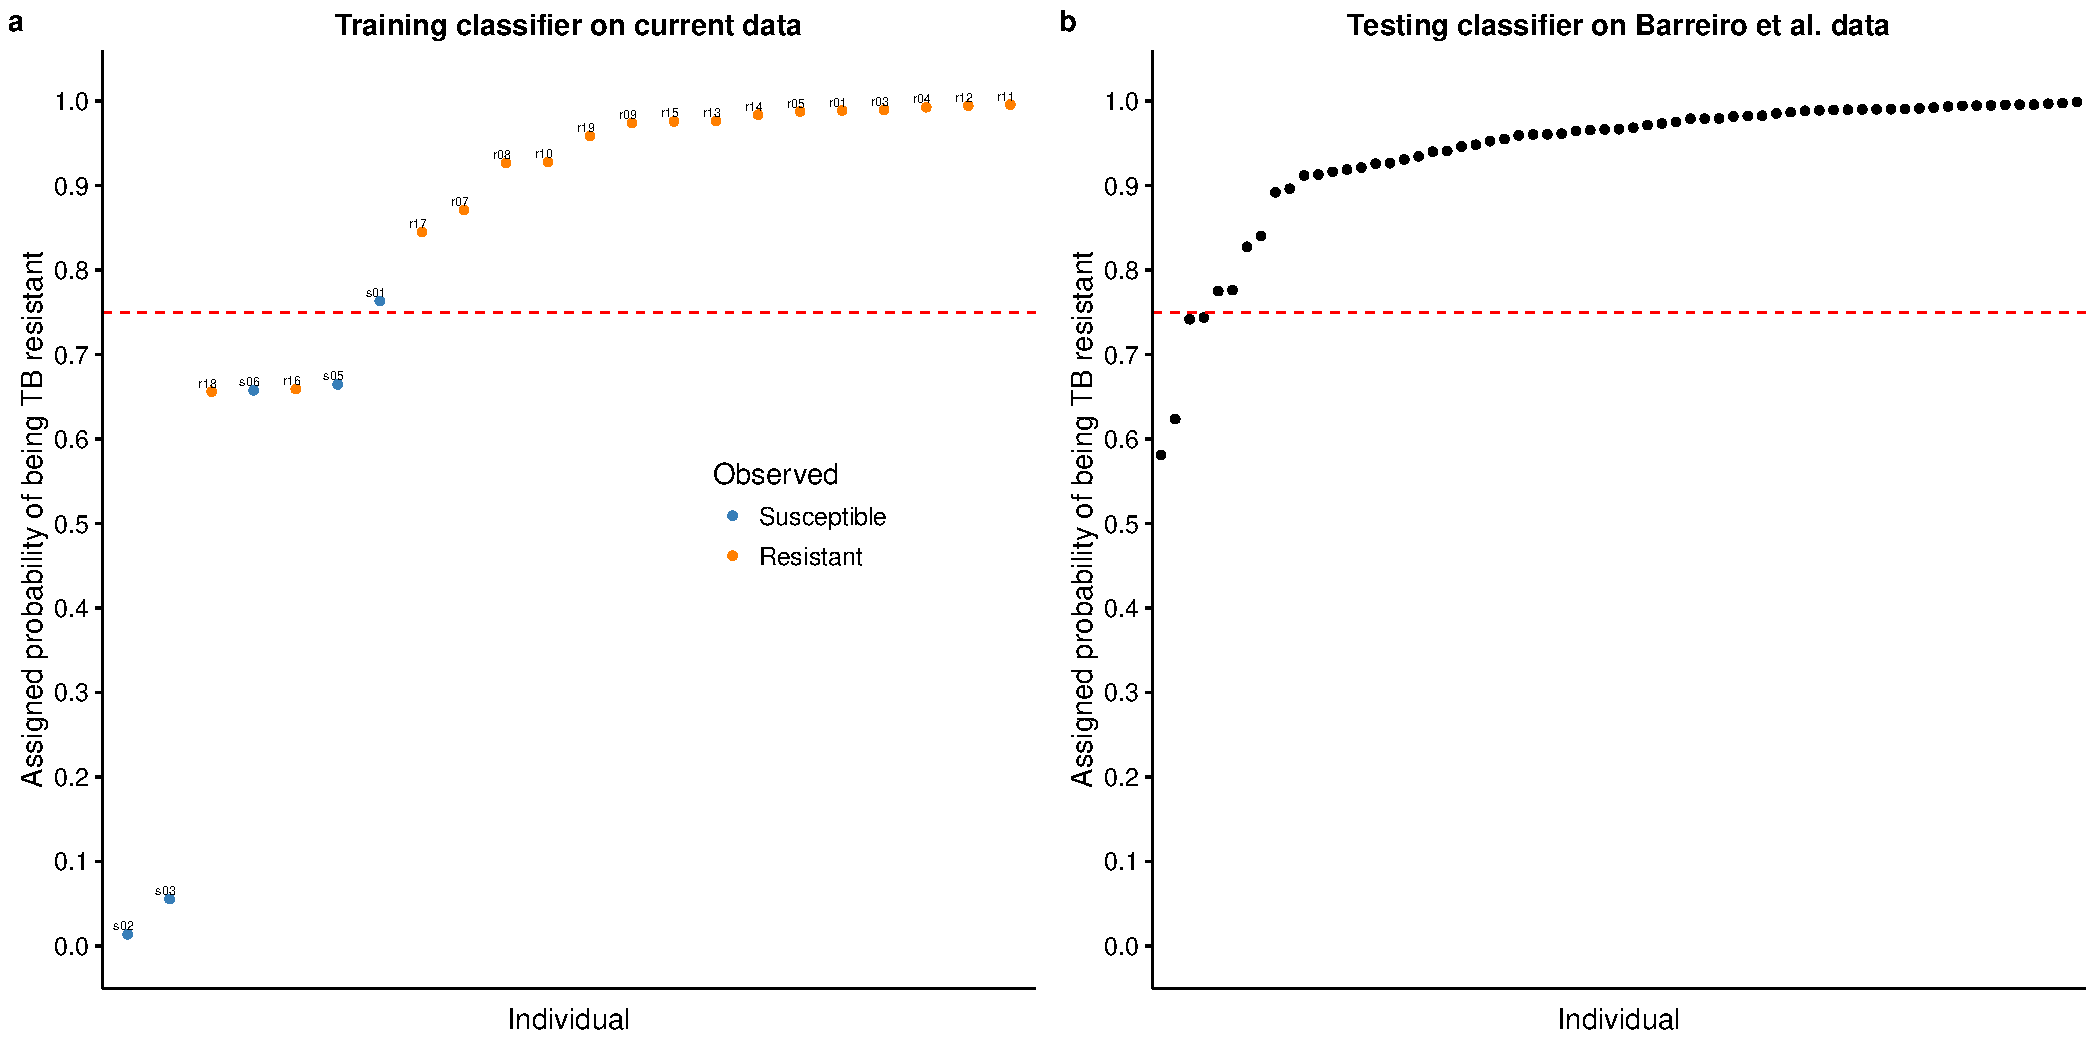
\includegraphics[width=\linewidth]{../figure/classifier-en.pdf}
\caption{
Classifying TB susceptible individuals using an elastic net model. (a)
The estimates of predicted probability of TB susceptibility from the
leave-one-out-cross-validation for individuals in the current study.
The blue circles represent individuals known to be susceptible to TB,
and orange those resistant to TB. The horizontal blue line at a
probability of 0.25 almost separates susceptible and resistant
individuals. (b) The estimates of predicted probability of TB
susceptibility from applying the classifier trained on the data from
the current study to a test set of independently collected healthy
individuals \cite{Barreiro2012}.
}
\label{fig:class-en}
\end{figure}

\begin{figure}[ht]
\centering
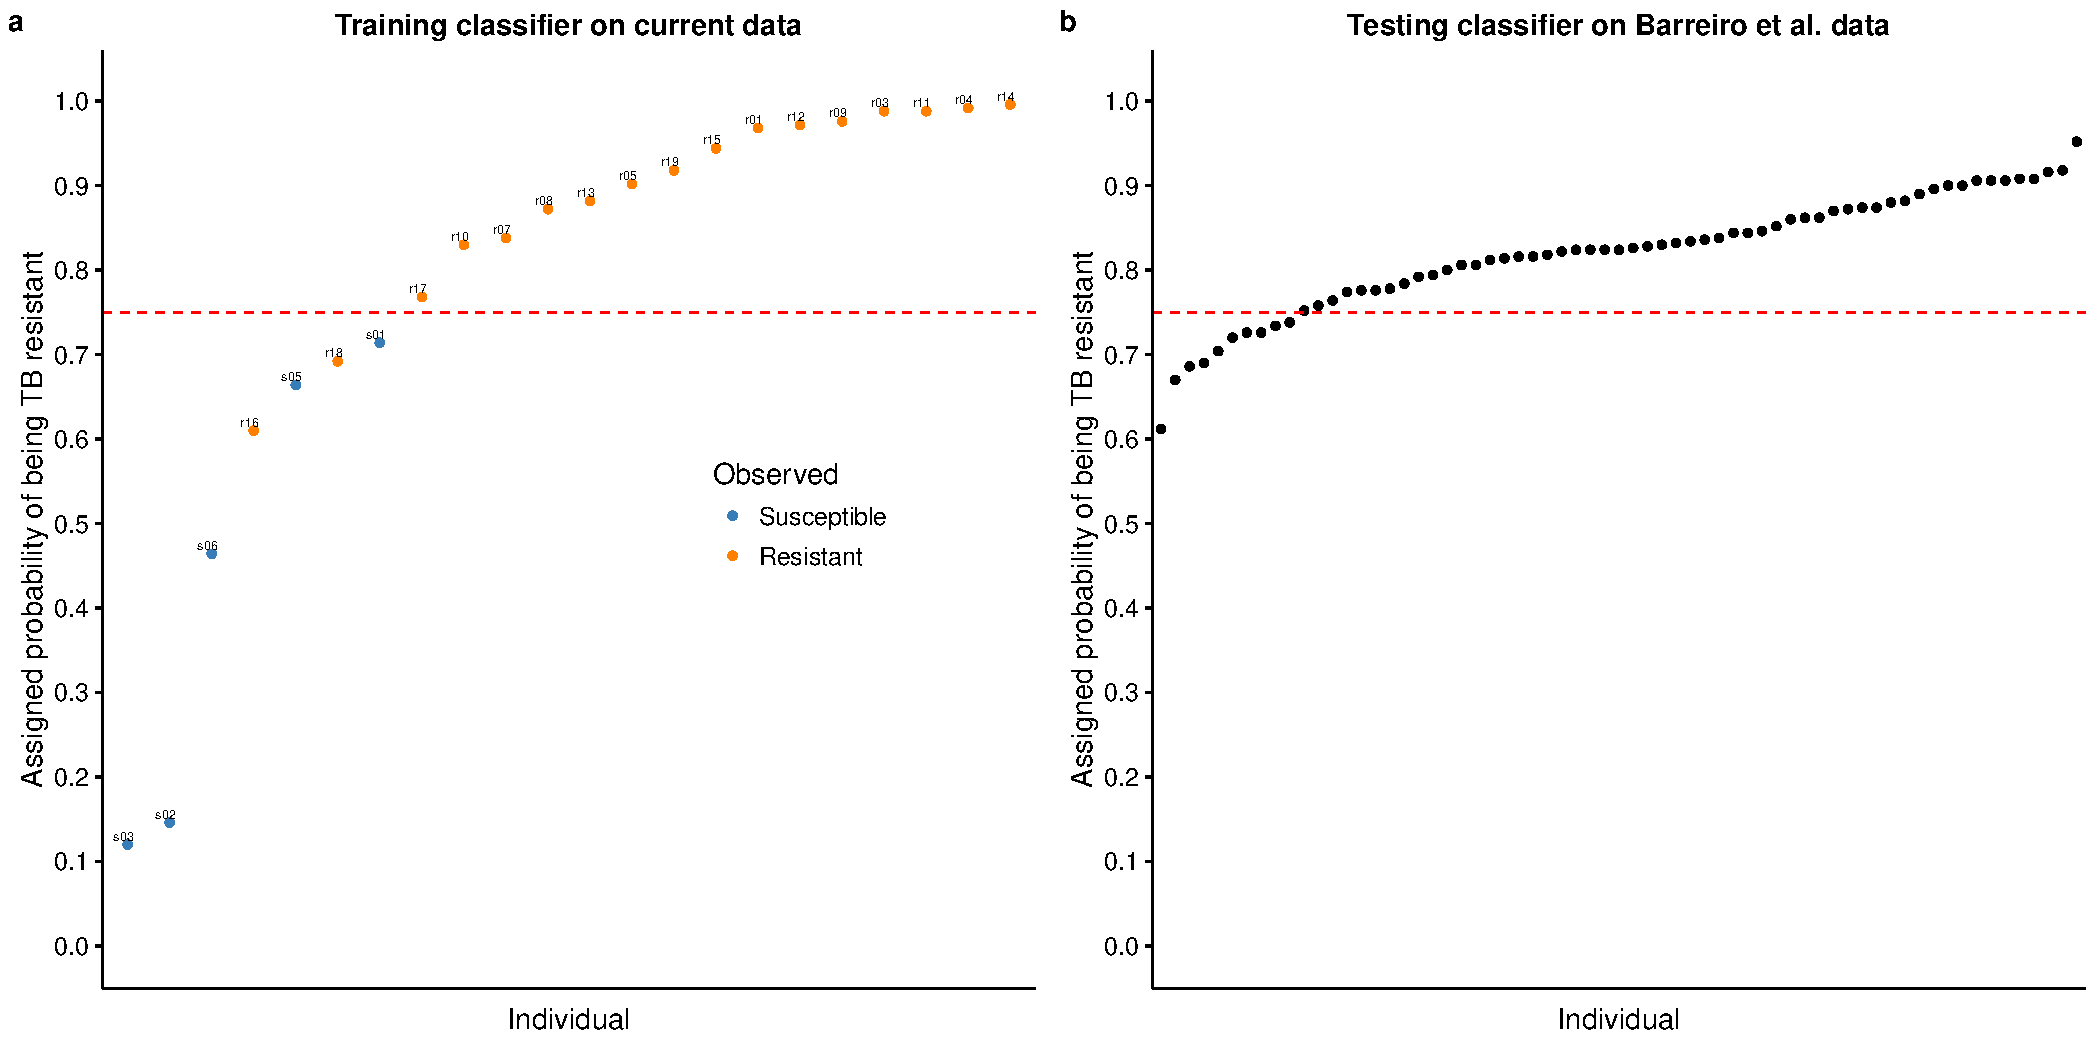
\includegraphics[width=\linewidth]{../figure/classifier-rf.pdf}
\caption{
Classifying TB susceptible individuals using a random forest model.
(a) The estimates of predicted probability of TB susceptibility from
the leave-one-out-cross-validation for individuals in the current
study. The blue circles represent individuals known to be susceptible
to TB, and orange those resistant to TB. The horizontal blue line at a
probability of 0.25 separates susceptible and resistant individuals.
(b) The estimates of predicted probability of TB susceptibility from
applying the classifier trained on the data from the current study to
a test set of independently collected healthy individuals
\cite{Barreiro2012}.
}
\label{fig:class-rf}
\end{figure}

\begin{figure}[ht]
\centering
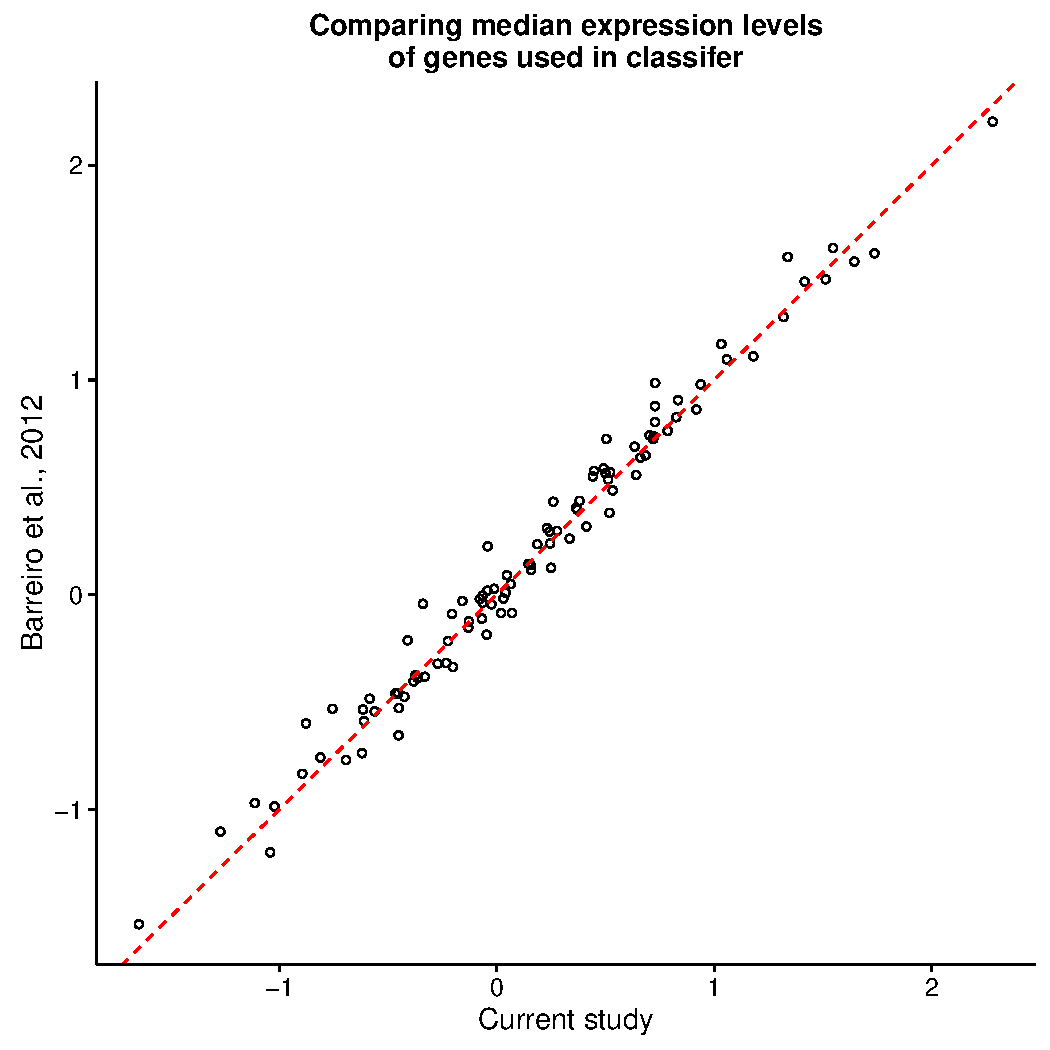
\includegraphics[width=4in]{../figure/classifier-exp.pdf}
\caption{
Comparing gene expression between the two studies. After normalization
and batch-correction, the median expression levels of the 99 genes
used in the classifier were similar between the samples in the current
study and those in Barreiro et al., 2012 \cite{Barreiro2012}. The
dashed red line is the 1:1 line.
}
\label{fig:class-exp}
\end{figure}

\begin{figure}[ht]
\centering
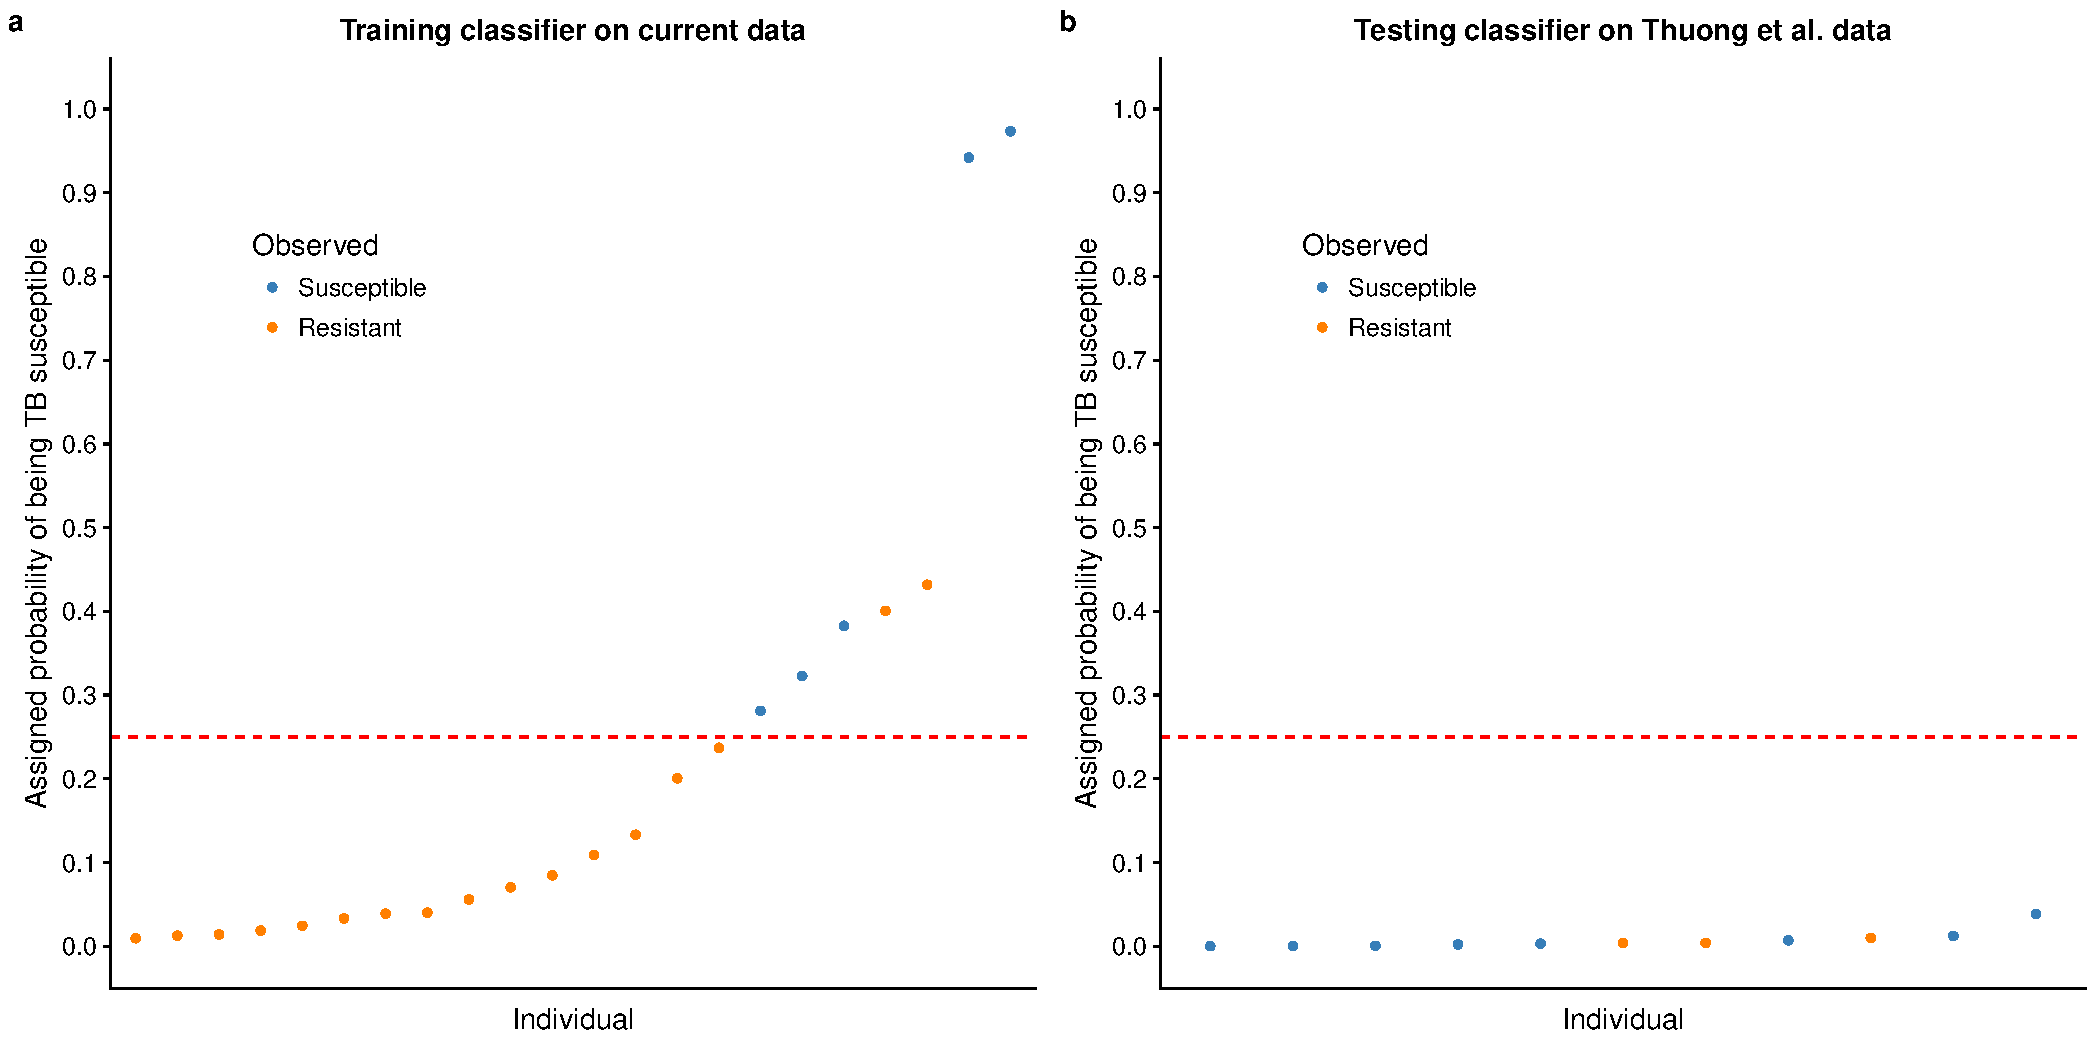
\includegraphics[width=\linewidth]{../figure/classifier-svm-thuong.pdf}
\caption{
Classifying individuals from Thuong et al., 2008\cite{Thuong2008}
using a support vector machine model. We followed the same training
and testing procedure performed for testing the classifier described
in the main text (Fig. \ref{fig:classifier}, see Classifier in
Methods). Not surprisingly since the data sets were from different
cell types, the classifier trained on the dendritic cells in this
study performed poorly when tested on samples with gene expression
levels measured in macrophages. To match our naming system, we labeled
the individuals from Thuong et al., 2008\cite{Thuong2008} with latent
TB as resistant (n = 3 after removing the outlier sample LTB2) and the
individuals recovered from pulmonary or meningeal TB as susceptible (n
= 4 each). (a) The estimates of predicted probability of TB
susceptibility from the leave-one-out-cross-validation for individuals
in the current study. The blue circles represent individuals known to
be susceptible to TB, and orange those resistant to TB. The horizontal
dashed red line at a probability of 0.25 separates susceptible and
resistant individuals. (b) The estimates of predicted probability of
TB susceptibility from applying the classifier trained on the data
from the current study to a test set of putatively susceptible and
resistant individuals \cite{Thuong2008}.
}
\label{fig:class-svm-thuong}
\end{figure}
\clearpage\newpage
\subsection*{Supplementary data}

\subsubsection*{Supplementary Data S1}

Supplementary Data S1 contains information on the 50 samples. Most
variables describe the batch processing steps outlined in
Supplementary Fig. \ref{fig:process}. “id” is a unique identifier for
each sample, “individual” is the individual identifier (“s” =
susceptible, “r” = resistant), “status” is the susceptibility status,
“treatment” is if the sample was infected or non-infected, “infection”
is the date of the infection experiment (12 total), “arrival” is the
identifier for the arrival batch (4 total), “extraction” is the batch
for RNA extraction (5 total), “master\_mix” is the batch for library
preparation (3 total), “rin” is the RNA Integrity Number from the
Agilent Bioanalyzer, and “outlier” is a Boolean variable indicating if
the sample was identified as an outlier (Supplementary Fig.
\ref{fig:outliers}) and removed from the analysis. (tds)
\subsubsection*{Supplementary Data S2}

Supplementary Data S2 contains the gene expression counts for the
11,336 genes after filtering lowly expressed genes for all 50 samples
(Supplementary Fig. \ref{fig:gene}). Each row is a gene labeled with
its Ensembl gene ID. Each column is a sample. Each sample is labeled
according to the pattern “x\#\#-status-treatment”, where x is “r” for
resistant or “s” for susceptible, \#\# is the ID number, status is
“resist” for resistant or “suscep” for susceptible, and treatment is
“noninf” for non-infected or “infect” for infected. (tds)
\subsubsection*{Supplementary Data S3}

Supplementary Data S3 contains the results of the differential
expression analysis with limma (Fig. \ref{fig:limma}). The workbook
contains 4 sheets corresponding to the 4 tests performed. “status\_ni”
is the test between resistant and susceptible individuals in the
non-infected state, “status\_ii” is the test between resistant and
susceptible individuals in the infected state, “treat\_resist” is the
test between the non-infected and infected states for resistant
individuals, and “treat\_suscep” is the test between the non-infected
and infected states for susceptible individuals. Each sheet has the
same columns. “id” is the Ensembl gene ID, “gene” is the gene name,
“logFC” is the log fold change from limma, “AveExpr” is the average
log expression from limma, “t” is the t-statistic from limma,
“P.Value” is the p-value from limma, “adj.P.Val” is the adjusted
p-value from limma, “qvalue” is the q-value calculated with adaptive
shrinkage, “chr” is the chromosome where the gene is located,
“description” is the description of the gene from Ensembl, “phenotype”
is the associated phenotype(s) assigned my Ensembl, “go\_id” is the
associated GO term(s) assigned by Ensembl, and “go\_description” is
the corresponding name(s) of the GO term(s). (xlsx)
\subsubsection*{Supplementary Data S4}

Supplementary Data S4 contains the results of the GWAS comparison
analysis (Fig. \ref{fig:gwas}). The first sheet “input-data” contains
the p-values for the GWAS SNP assigned to each gene from each study.
The columns “gwas\_p\_russia”, “gwas\_p\_gambia”, “gwas\_p\_ghana”,
“gwas\_p\_uganda”, “gwas\_p\_height” contain the p-values from the TB
susceptibility GWAS in Russia, The Gambia, Ghana, Uganda and Tanzania,
and the height GWAS in Europeans, respectively. The columns
“status\_ni”, “status\_ii”, “treat\_resist”, and “treat\_suscep” refer
to the tests described for Supplementary Data S3 and contain the log
fold changes for each comparison. All the other gene annotation
columns are the same as described for Supplementary Data S3. The
second sheet “top-genes” contains a subset of the full results to
highlight those genes which had an absolute log fold change greater
than 2 between resistant and susceptible individuals in the
non-infected state (“status\_ni”). (xlsx)
\subsubsection*{Supplementary Data S5}

Supplementary Data S5 contains the results of the classifier analysis.
Specifically it contains the results from the support vector machine
using the genes with a q-value less than 0.05 (Fig.
\ref{fig:classifier}). The sheet “gene-list” contains information
about the genes used for the classifier (the columns are described in
the section for Supplementary Data S3). The sheet “training-input”
contains the input gene expression data for training the model. The
sheet “training-results” contains the results of the
leave-one-out-cross-validation when training the model on the samples
from the current study. The sheet “testing-input” contains the input
gene expression data for testing the model. The sheet
“testing-results” contains the results from testing the model on the
samples from Barreiro et al., 2012 \cite{Barreiro2012}. The column
“prob\_tb\_suscep” is the probability of being susceptible to TB
assigned by the model. (xlsx)
\end{document}
